% !TEX root = ./main.tex
\documentclass[10pt,a4paper]{article}

\usepackage[spanish,es-tabla]{babel}
\usepackage[margin=2.0cm]{geometry}
\usepackage{amsmath, amsfonts, amssymb}
\usepackage{graphicx}
\usepackage{hyperref}
\usepackage{booktabs}
\usepackage{xcolor}
\usepackage{enumitem}

\graphicspath{{Imagenes/}}

\setlist{itemsep=2pt, topsep=3pt, parsep=1pt}
\emergencystretch=1.5em
\setlength{\textfloatsep}{8pt plus 2pt minus 2pt}
\setlength{\floatsep}{6pt plus 2pt minus 2pt}
\setlength{\intextsep}{6pt plus 2pt minus 2pt}

\hypersetup{
    colorlinks=true,
    linkcolor=blue,
    filecolor=magenta,
    urlcolor=cyan,
    citecolor=blue,
    hypertexnames=false,
}

\begin{document}
\pagenumbering{roman}

\begin{titlepage}
    \centering
    
\includegraphics[width=0.22\textwidth]{logoUV.jpg}\par\vspace{0.8cm}
    {\scshape\LARGE Universidad del Valle \par}
    \vspace{0.3cm}
    {\scshape\Large Escuela de Ingeniería de Sistemas y Computación \par}
    \vspace{0.3cm}
    {\scshape\large Programación por Restricciones \par}
    \vspace{1.2cm}
    {\huge\bfseries Proyecto de Curso: Planificación de los Ensayos en una Telenovela (COP) \par}
    \vspace{1.2cm}
    {\Large\textbf{Integrantes:}\par}
    \vspace{0.4cm}
    {\large
    Cristian David Cabrera Pantoja\\
    Junior Orlando Cantor Arevalo\\
    Juan Diego Cárdenas Mejía\par}
    \vfill
    {\large \textbf{Profesor:} Robinson Duque \par}
    \vspace{0.8cm}
    {\large Cali, Colombia \\ \today \par}
\end{titlepage}

\tableofcontents
\newpage
\pagenumbering{arabic}

% !TEX root = ../main.tex
\section{Parte 1: Modelo COP de Planificación de Ensayos}
\label{sec:modelo_parte1}

La planificación del orden de grabación de las escenas de una telenovela se formula como un Problema de Optimización con Restricciones sobre dominios enteros finitos ($\text{COP}(\mathcal{FD})$), dado por $\mathcal{P}_1 = \langle \mathcal{X}_1, \mathcal{D}_1, \mathcal{C}_1, f_1 \rangle$. Cada actor cobra por unidad de tiempo continua de permanencia en el estudio, contada desde el inicio de la primera escena en que participa hasta la finalización de la última; el objetivo es hallar una permutación de las escenas que minimice el costo salarial total.

\subsection{Conjuntos y Parámetros}

El modelo se parametriza a partir de los tres elementos normalizados del archivo de entrada (\texttt{*.dzn}), sin constantes fijas de dimensión:
\begin{itemize}
    \item \textbf{Conjuntos:} $A = \{1, \dots, N\}$ (\texttt{ACTORES}, preservando el orden nominal de entrada, $N = |A| \in \mathbb{Z}^+$); $E = \{1, \dots, M\}$ (escenas, con $M = |\texttt{Duracion}| \in \mathbb{Z}^+$); y $K = \{1, \dots, M\}$ (posiciones o turnos secuenciales de grabación).
    \item \textbf{Parámetros de entrada:} $p_{a,e} \in \{0, 1\}$ (\texttt{Escenas[a, e]}), igual a $1$ si el actor $a$ interviene en la escena $e$ y $0$ en otro caso; $c_a \in \mathbb{Z}_{\ge 0}$ (\texttt{Escenas[a, M+1]}), tarifa salarial del actor $a$ (cientos de miles de pesos por unidad de tiempo); y $d_e \in \mathbb{Z}^+$ (\texttt{Duracion[e]}), duración de la escena $e$.
    \item \textbf{Parámetros derivados en compilación:}
    \begin{align}
        D_{\text{total}} &= \sum_{e \in E} d_e, \qquad
        E_a = \{e \in E \mid p_{a,e} = 1\}, \qquad
        K_a = |E_a| = \sum_{e \in E} p_{a,e} \label{eq:p1_derivados1} \\
        D^{\min}_a &= \sum_{e \in E_a} d_e, \qquad
        U^{(1)}_a = \begin{cases} D_{\text{total}}, & \text{si } K_a > 0 \\ 0, & \text{si } K_a = 0 \end{cases}, \qquad
        C_{\text{fijo}} = \sum_{a \in A} c_a \cdot D^{\min}_a \label{eq:p1_derivados2}
    \end{align}
    donde $D_{\text{total}}$ es el horizonte total de rodaje, $E_a$ el subconjunto de escenas del actor $a$, $D^{\min}_a$ su tiempo efectivo de actuación y $C_{\text{fijo}}$ la cota salarial inferior alcanzable únicamente sin esperas. Sea además $d^{\uparrow}_1 \le d^{\uparrow}_2 \le \dots \le d^{\uparrow}_M$ el vector $d$ ordenado ascendentemente.
\end{itemize}

\subsection{Variables de Decisión y Dominios}

Separando parámetros conocidos de incógnitas y aplicando consistencia de nodo inicial (Capítulo 5 de Apt) para excluir desde la raíz valores imposibles, se definen:
\begin{enumerate}
    \item \textbf{Secuencia primal ($Orden_k$, $k \in K$) y posición dual ($Pos_e$, $e \in E$):} Escena asignada al turno $k$ y turno en que se graba la escena $e$:
    \begin{equation}
        D(Orden_k) = E = \{1, \dots, M\} \;\; (\forall k \in K), \qquad
        D(Pos_e) = K = \{1, \dots, M\} \;\; (\forall e \in E)
        \label{eq:dom_orden_pos}
    \end{equation}
    \item \textbf{Tiempo acumulado ($Acum_k$, $k \in \{0, \dots, M\}$):} Instante en que concluye el turno $k$ ($Acum_0 = 0$). Las primeras $k$ escenas suman al menos las $k$ duraciones menores y a lo sumo las $k$ mayores:
    \begin{equation}
        D(Acum_k) = \left[\sum_{j=1}^{k} d^{\uparrow}_j \;\dots\; \sum_{j=M-k+1}^{M} d^{\uparrow}_j\right] \subseteq [0 \dots D_{\text{total}}], \quad \forall k \in \{0, \dots, M\}
        \label{eq:dom_acum}
    \end{equation}
    \item \textbf{Turnos extremos por actor ($primera_a, ultima_a$, $a \in A$):} Primer y último turno donde actúa $a$. Si $K_a > 0$, tras $primera_a$ deben caber al menos las restantes $K_a - 1$ escenas de $E_a$ y hasta $ultima_a$ deben haberse filmado al menos $K_a$ escenas propias (fijándose a $\{1\}$ si $K_a = 0$):
    \begin{equation}
        D(primera_a) = \{1, \dots, M - K_a + 1\}, \qquad
        D(ultima_a) = \{K_a, \dots, M\} \quad (K_a > 0)
        \label{eq:dom_prim_ult}
    \end{equation}
    \item \textbf{Ingreso, salida, permanencia y espera ($ini_a, fin_a, tiempo_a, espera_a$, $a \in A$):} Instantes de llegada y retiro del estudio, estadía continua total y tiempo sin actuar dentro del set. Como tras $ini_a$ resta al menos $D^{\min}_a$ de actuación propia y antes de $fin_a$ transcurre al menos $D^{\min}_a$ (con dominio $\{0\}$ si $K_a = 0$):
    \begin{align}
        D(ini_a) &= [0 \dots D_{\text{total}} - D^{\min}_a], &
        D(fin_a) &= [D^{\min}_a \dots D_{\text{total}}] \nonumber \\
        D(tiempo_a) &= [D^{\min}_a \dots U^{(1)}_a], &
        D(espera_a) &= [0 \dots U^{(1)}_a - D^{\min}_a]
        \label{eq:dom_tiempo_espera}
    \end{align}
    \item \textbf{Costo salarial total ($Costo$):} Variable objetivo con techo $\overline{C}_1 = \sum_{a \in A} c_a U^{(1)}_a$:
    \begin{equation}
        D(Costo) = [C_{\text{fijo}} \dots \overline{C}_1]
        \label{eq:dom_costo_p1}
    \end{equation}
\end{enumerate}

\subsection{Restricciones Primarias y Función Objetivo}

El conjunto $\mathcal{C}_1 = \{C_1, C_2, C_3\}$ se formula sin condicionar sobre valores individuales de variables de decisión:
\begin{enumerate}
    \item \textbf{Biyección turno-escena ($C_1$):} Cada escena ocupa un único turno y $Orden$, $Pos$ son permutaciones inversas mutuas:
    \begin{equation}
        \forall j < k \in K:\; Orden_j \neq Orden_k, \qquad
        \forall k \in K:\; Pos_{Orden_k} = k, \qquad
        \forall e \in E:\; Orden_{Pos_e} = e
        \label{eq:c1_inverse}
    \end{equation}
    \emph{Semántica:} Impide omitir o repetir escenas y enlaza la consulta por turno con la consulta por escena.

    \item \textbf{Cronología acumulada ($C_2$):} El reloj del estudio avanza sin huecos en la duración de cada escena:
    \begin{equation}
        Acum_0 = 0, \qquad Acum_M = D_{\text{total}}, \qquad
        \forall k \in K: \; Acum_k = Acum_{k-1} + d_{Orden_k}
        \label{eq:c2_acum}
    \end{equation}
    \emph{Semántica:} El turno $k$ se ejecuta durante el intervalo $[Acum_{k-1}, Acum_k]$ de longitud $d_{Orden_k}$.

    \item \textbf{Permanencia y espera por actor ($C_3$):} Para todo $a \in A$ con $K_a > 0$ (y $0$ cuando $K_a = 0$):
    \begin{align}
        primera_a &= \min_{e \in E_a} Pos_e, &
        ultima_a &= \max_{e \in E_a} Pos_e, &
        ini_a &= Acum_{primera_a - 1} \label{eq:c3_extremos} \\
        fin_a &= Acum_{ultima_a}, &
        tiempo_a &= fin_a - ini_a, &
        espera_a &= tiempo_a - D^{\min}_a \label{eq:c3_tiempo}
    \end{align}
    \emph{Semántica:} $Acum_{primera_a - 1}$ marca el inicio de $primera_a$ y $Acum_{ultima_a}$ el término de $ultima_a$; su resta mide la estadía continua del actor en el set.
\end{enumerate}

La función objetivo $f_1$ minimiza el pago total al elenco:
\begin{equation}
    \text{Minimizar } Costo = \sum_{a \in A} c_a \cdot tiempo_a
    \label{eq:obj_p1}
\end{equation}
\emph{Adecuación y búsqueda:} (i) Para cualquier permutación $\pi$, la suma telescópica $Acum_{ultima_a} - Acum_{primera_a - 1} = \sum_{k=primera_a}^{ultima_a} d_{\pi_k}$ calcula el cobro exacto (p.\ ej., en $\pi = (1,\dots,20)$ de ``Desenfreno de Pasiones'', para el Actor 3 da $primera_3 = 2$, $ultima_3 = 15$, $tiempo_3 = 21 - 2 = 19$ y costo $19 \times 5 = 95$); (ii) definir $primera_a$ y $ultima_a$ sobre el conjunto estático $E_a$ evita matrices booleanas reificadas; y (iii) separar $espera_a = tiempo_a - D^{\min}_a$ aísla el sobrecosto variable. La resolución usa \emph{Branch-and-Bound} sobre los turnos intercalados desde los extremos ($1, M, 2, M-1, \dots$) probando primero escenas de menor peso salarial ($E_1$, Sección~\ref{sec:busqueda}).

% !TEX root = ../main.tex
\section{Parte 2: Disponibilidad, Conflictos (\texttt{Evitar}) y Objetivo Jerárquico}
\label{sec:modelo_parte2}

La Parte 2 extiende $\mathcal{P}_1$ al modelo $\mathcal{P}_2 = \langle \mathcal{X}_2, \mathcal{D}_2, \mathcal{C}_2, f_2 \rangle$, incorporando topes contractuales de tiempo máximo en el estudio por actor (\texttt{Disponibilidad}) y pares de actores cuya coincidencia simultánea en el estudio debe reducirse (\texttt{Evitar}), dando prioridad absoluta a minimizar primero el costo salarial.

\subsection{Parámetros, Variables y Dominios Adicionales}

A los datos de la Parte 1 se suman dos tablas de entrada:
\begin{itemize}
    \item \textbf{Disponibilidad por actor (\texttt{Disponibilidad}):} Relación de $N$ pares $(\text{actor}, \text{límite})$ asociada a cada $a \in A$ como $Disp_a \in \mathbb{Z}_{\ge 0}$ sin depender del orden de filas en el archivo \texttt{.dzn}. El valor $Disp_a = 0$ indica tiempo ilimitado y $Disp_a > 0$ fija la permanencia máxima admisible, ajustando la cota superior $U^{(2)}_a$ desde la raíz:
    \begin{equation}
        U^{(2)}_a = \begin{cases}
            0, & \text{si } K_a = 0 \\
            \min(D_{\text{total}}, Disp_a), & \text{si } K_a > 0 \land Disp_a > 0 \\
            D_{\text{total}}, & \text{si } K_a > 0 \land Disp_a = 0
        \end{cases}
        \label{eq:u2_actor}
    \end{equation}
    Si $Disp_a > 0$ y $D^{\min}_a > Disp_a$, la instancia es infactible y es rechazada por aserción estática. Si $Disp_a = D^{\min}_a$ (Actor 7 en \texttt{Desenfreno4.dzn}: $D^{\min}_7 = Disp_7 = 5$), el dominio se reduce en compilación a $D(tiempo_7) = \{5\}$ y $D(espera_7) = \{0\}$.
    \item \textbf{Pares a evitar (\texttt{Evitar}):} Lista $P_{\text{ev}} = \{1, \dots, L\}$ ($L \ge 0$, admitiendo $L = 0$) de pares $(a_{p,1}, a_{p,2}) \in A^2$ con $a_{p,1} \neq a_{p,2}$, con cotas estáticas de coincidencia:
    \begin{equation}
        \underline{\tau}_p = \sum_{e \in E_{a_{p,1}} \cap E_{a_{p,2}}} d_e, \qquad
        \overline{\tau}_p = \min\big(U^{(2)}_{a_{p,1}},\; U^{(2)}_{a_{p,2}}\big), \quad \forall p \in P_{\text{ev}}
        \label{eq:cotas_solape}
    \end{equation}
\end{itemize}

Conservando $\mathcal{X}_1$ con $U^{(2)}_a$ y $\overline{C}_2 = \sum_{a \in A} c_a U^{(2)}_a$, se agregan las variables:
\begin{enumerate}
    \item \textbf{Solape por par ($solape_p$, $p \in P_{\text{ev}}$):} Tiempo simultáneo en estudio de $a_{p,1}$ y $a_{p,2}$, con $D(solape_p) = [\underline{\tau}_p \dots \overline{\tau}_p]$.
    \item \textbf{Tiempo compartido total ($TiempoCompartido$):} Variable $TC$ con dominio $[\underline{TC} \dots \overline{TC}]$, donde $\underline{TC} = \sum_{p \in P_{\text{ev}}} \underline{\tau}_p$ y $\overline{TC} = \sum_{p \in P_{\text{ev}}} \overline{\tau}_p$ ($\{0\}$ si $P_{\text{ev}} = \emptyset$).
    \item \textbf{Objetivo lexicográfico ($ObjetivoLex$):} Entero con dominio $[W \cdot C_{\text{fijo}} + \underline{TC} \;\dots\; W \cdot \overline{C}_2 + \overline{TC}]$, donde $W = \overline{TC} + 1$.
\end{enumerate}

\subsection{Restricciones Adicionales y Función Objetivo Lexicográfica}

Al sistema $\{C_1, C_2, C_3\}$ se añaden $C_4$ y $C_5$:
\begin{enumerate}
    \setcounter{enumi}{3}
    \item \textbf{Tope de disponibilidad ($C_4$):} Ningún actor con límite activo puede superar su tiempo pactado en el set:
    \begin{equation}
        \forall a \in A \text{ con } Disp_a > 0: \quad tiempo_a \le Disp_a
        \label{eq:c4_disp}
    \end{equation}
    \emph{Semántica:} Restringe la cantidad de escenas ajenas intercalables entre la primera y la última aparición de $a$.

    \item \textbf{Intersección temporal de estadías para \texttt{Evitar} ($C_5$):} Para todo par $p = (a_{p,1}, a_{p,2}) \in P_{\text{ev}}$ con ambos actores activos ($solape_p = 0$ si alguno verifica $K_a = 0$), el cruce de sus estadías continuas viene dado por:
    \begin{align}
        solape_p &= \max\Big(0,\; \min\big(fin_{a_{p,1}}, fin_{a_{p,2}}\big) - \max\big(ini_{a_{p,1}}, ini_{a_{p,2}}\big)\Big) \label{eq:c5_evitar} \\
        TC &= \sum_{p \in P_{\text{ev}}} solape_p \label{eq:tc_suma}
    \end{align}
    \emph{Semántica:} Si un actor sale antes de que el otro ingrese, la diferencia es no positiva y $solape_p = 0$; si sus estadías se cruzan (actuando juntos o esperando en paralelo), $solape_p$ mide la longitud exacta del traslape.
\end{enumerate}

Para optimizar jerárquicamente $Costo$ en primer nivel y $TC$ en segundo nivel en una sola ejecución, se minimiza:
\begin{equation}
    \text{Minimizar } ObjetivoLex = W \cdot Costo + TC, \qquad W = \overline{TC} + 1
    \label{eq:obj_lex}
\end{equation}
\emph{Prueba de equivalencia lexicográfica:} Para dos soluciones factibles $\pi_1, \pi_2$, se cumple $0 \le TC \le \overline{TC} = W - 1$, luego $|TC(\pi_2) - TC(\pi_1)| \le W - 1$. (i) Si $Costo(\pi_1) < Costo(\pi_2)$, por integridad $Costo(\pi_2) - Costo(\pi_1) \ge 1$ y $ObjetivoLex(\pi_2) - ObjetivoLex(\pi_1) \ge W - (W - 1) = 1 > 0$, prefiriéndose siempre $\pi_1$ sin importar $TC$. (ii) Si $Costo(\pi_1) = Costo(\pi_2)$, entonces $ObjetivoLex(\pi_1) < ObjetivoLex(\pi_2) \iff TC(\pi_1) < TC(\pi_2)$. La cota ajustada $W = \overline{TC} + 1$ evita desbordamiento en enteros de 32 bits (en \texttt{Desenfreno4.dzn}, $W = 101$ y $ObjetivoLex^* = 101 \times 880 + 37 = 88\,917 \ll 2^{31}-1$). La búsqueda aplica igualmente $E_1$ (\emph{Outside-In} por peso salarial ascendente), cerrando temprano $primera_a$ y $ultima_a$ para activar $C_4$ y $C_5$.

% !TEX root = ../main.tex
\section{Detalles de Implementación: Eliminación de Simetrías y Restricciones Redundantes}
\label{sec:implementacion}

Las implementaciones modulares de la Parte 1 (\nolinkurl{problemas/parte1/TelenovelaParte1.mzn}) y de la Parte 2 (\nolinkurl{problemas/parte2/TelenovelaParte2.mzn}) materializan fielmente los modelos $\mathcal{P}_1$ y $\mathcal{P}_2$ sin introducir constantes fijas de dimensión, validando mediante aserciones estáticas la positividad de \texttt{Duracion}, el carácter binario de \texttt{Escenas}, la no negatividad de tarifas y disponibilidades, la biyección completa de actores en \texttt{Disponibilidad} y la factibilidad elemental $D^{\min}_a \le Disp_a$. Esta sección expone, sin incluir código fuente, las decisiones estructurales clave de implementación: canalización primal-dual, eliminación formal de simetrías con recuperación algebraica de soluciones, restricciones redundantes de fortalecimiento de cotas e interfaz gráfica y normalizada de entrada/salida.

\subsection{Canalización Primal-Dual y Representación sin Multiplicación de Variables}

En problemas de secuenciación con duraciones heterogéneas $d_e \neq 1$, una formulación ingenua basada únicamente en indicadores booleanos de presencia por turno $en\_set_{a,k} \in \{0,1\}$ exigiría evaluar productos cuadráticos entre dos incógnitas ($d_{Orden_k} \cdot en\_set_{a,k}$) en cada posición $k \in K$, degradando severamente la propagación lineal. La arquitectura adoptada resuelve esta dificultad combinando dos vistas canalizadas mediante la restricción global \texttt{inverse} (consistente en dominio):
\begin{enumerate}
    \item La vista por posiciones $Orden_k$ alimenta mediante restricciones globales \texttt{element} la recurrencia lineal de tiempos acumulados $Acum_k = Acum_{k-1} + d_{Orden_k}$.
    \item La vista dual por escenas $Pos_e$ permite obtener $primera_a$ y $ultima_a$ aplicando directamente los propagadores globales \texttt{minimum} y \texttt{maximum} sobre el subarreglo de variables indexado por el conjunto constante $E_a$, tras lo cual un segundo par de restricciones \texttt{element} ($ini_a = Acum_{primera_a - 1}$ y $fin_a = Acum_{ultima_a}$) determina exactamente la estadía en tiempo continuo sin productos no lineales.
\end{enumerate}

\subsection{Análisis, Eliminación de Simetrías y Recuperación de Soluciones}
\label{subsec:simetrias}

Un automorfismo de simetría de un COP de secuenciación es una transformación biyectiva sobre el espacio de permutaciones $\mathfrak{S}_M$ que preserva invariantes todas las restricciones primarias ($C_1$--$C_5$) y los valores objetivos ($Costo$ y $TiempoCompartido$). El análisis estructural del problema revela tres familias independientes de simetrías ($S_1$, $S_2$ y $S_3$):

\begin{enumerate}
    \item \textbf{Fijación canónica en prefijo de escenas sin participación actoral ($S_3$):}
    Sea $E_{\emptyset} = \{e \in E \mid \forall a \in A,\; p_{a,e} = 0\} = \{e^{(0)}_1 < e^{(0)}_2 < \dots < e^{(0)}_q\}$ el subconjunto ordenado de escenas en las que no interviene ningún actor del elenco (por ejemplo, la escena $1$ en \texttt{Trivial1.dzn}, o las escenas $2$ y $7$ en \texttt{Instancia01\_P1.dzn}). Insertar cualquier escena $e_0 \in E_{\emptyset}$ dentro del intervalo activo $[primera_a, ultima_a]$ de un actor solo incrementa artificialmente su espera en $+d_{e_0}$; en cambio, ubicar las $q$ escenas vacías fuera de todos los intervalos actorales (al principio o al final del rodaje, en cualquiera de sus $q!$ órdenes internos) traslada todos los intervalos $[ini_a, fin_a]$ por una misma constante aditiva $\delta$, dejando idénticas todas las diferencias $tiempo_a = fin_a - ini_a$ y todas las intersecciones temporales de \texttt{Evitar}. Para eliminar las $q!$ permutaciones internas y los desplazamientos de borde entre prefijo y sufijo, se fijan canónicamente en las primeras $q$ posiciones:
    \begin{equation}
        \forall j \in \{1, \dots, q\}: \quad Orden_j = e^{(0)}_j
        \label{eq:s3_vacias}
    \end{equation}
    Además de podar un factor de al menos $q! \cdot 2^q$ ramas equivalentes, $S_3$ resulta indispensable para que la ruptura de inversión temporal $S_1$ no sea neutralizada cuando una escena vacía de índice mínimo ocupa $Orden_1$.

    \item \textbf{Simetría global de inversión temporal del cronograma ($S_1$):}
    Sea $\pi$ un cronograma con las escenas vacías en $1..q$ y las $M - q$ escenas activas en $q+1..M$. Considérese la permutación especular $\pi^{\text{rev}}$ obtenida al invertir únicamente el subarreglo activo $(\pi_{q+1}, \dots, \pi_M)$. Para cada actor activo $a \in A$, el inicio y el fin de su estadía pasan a ubicarse en las posiciones simétricas $M + q + 1 - ultima_a(\pi)$ y $M + q + 1 - primera_a(\pi)$, abarcando exactamente el mismo multiconjunto de escenas en orden inverso. Por consiguiente, la duración $tiempo_a$ permanece idéntica para todo actor (preservando $Costo$ y $Disponibilidad$), y en todo par conflictivo de \texttt{Evitar} la intersección de estadías coincide, manteniendo invariantes $solape_p$ y $TC$. Como $\pi_{q+1} \neq \pi_M$ siempre que $M - q \ge 2$, exactamente uno de los dos cronogramas satisface la desigualdad estricta:
    \begin{equation}
        M - q \ge 2 \implies Orden_{q+1} < Orden_M
        \label{eq:s1_inversion}
    \end{equation}
    reduciendo exactamente a la mitad el espacio de búsqueda sobre las escenas con elenco.

    \item \textbf{Simetría de permutación entre escenas gemelas ($S_2$):}
    Dos escenas distintas $e_1 < e_2 \in E$ son \emph{indistinguibles o gemelas} si exigen exactamente el mismo subconjunto de actores ($\forall a \in A,\; p_{a, e_1} = p_{a, e_2}$) y poseen idéntica duración ($d_{e_1} = d_{e_2}$), como sucede con las escenas $3$ y $4$ en \texttt{Trivial1.dzn} y \texttt{Trivial2.dzn}. Nótese que ambas condiciones son necesarias: si difiriesen en duración ($d_{e_1} \neq d_{e_2}$), intercambiarlas cuando solo una de ellas cae dentro del intervalo de espera de un tercer actor alteraría la estadía de dicho tercer actor. Cuando se cumplen ambas igualdades, la transposición $(e_1\; e_2)$ deja invariantes $primera_a$, $ultima_a$, $Acum_k$, $Costo$, $Disponibilidad$ y $TC$. Esta simetría de valor se rompe imponiendo orden creciente de posición sobre las escenas gemelas:
    \begin{equation}
        \forall e_1 < e_2 \in E \text{ tales que } d_{e_1} = d_{e_2} \land (\forall a \in A,\; p_{a,e_1} = p_{a,e_2}): \quad Pos_{e_1} < Pos_{e_2}
        \label{eq:s2_gemelas}
    \end{equation}
\end{enumerate}

\paragraph{Recuperación exacta de las soluciones simétricas eliminadas.}
Sea $\pi^*$ una solución óptima canónica obtenida bajo $S_1 \land S_2 \land S_3$, y particiónense las escenas activas $E \setminus E_{\emptyset}$ en clases de equivalencia de escenas gemelas $G_1, G_2, \dots, G_r$. Toda la órbita de soluciones óptimas equivalentes descartadas se reconstruye de forma cerrada y sin re-ejecutar el solver mediante tres operaciones algebraicas:
\begin{enumerate}
    \item \emph{Acción de los grupos simétricos de escenas gemelas ($S_2$):} Aplicar sobre las etiquetas de $\pi^*[q+1..M]$ cualquiera de las $\prod_{\ell=1}^r |G_\ell|!$ permutaciones internas del grupo producto $\prod_{\ell=1}^r \mathfrak{S}_{|G_\ell|}$ (por ejemplo, intercambiar las escenas $3$ y $4$ en $[3, 4, 6, 2, 1, 5]$ recupera inmediatamente la solución $[4, 3, 6, 2, 1, 5]$ de \texttt{Trivial2.dzn}).
    \item \emph{Reflexión temporal del bloque activo ($S_1$):} Para cada secuencia generada en el paso anterior, invertir el subarreglo activo $(\pi_{q+1}, \dots, \pi_M) \mapsto (\pi_M, \dots, \pi_{q+1})$, duplicando la cardinalidad de la órbita (por ejemplo, $[4, 3, 6, 2, 1, 5] \mapsto [5, 1, 2, 6, 3, 4]$).
    \item \emph{Reubicación de borde de escenas vacías ($S_3$):} Distribuir libremente las $q$ escenas de $E_{\emptyset}$ entre el prefijo (antes de la primera escena activa) y el sufijo (después de la última escena activa) en cualquiera de sus $q!$ permutaciones, generando un total de $(q + 1)! / 1 = q! \cdot (q + 1)$ disposiciones de borde equivalentes en costo y solape.
\end{enumerate}

\subsection{Restricciones Redundantes y Justificación de Poda}
\label{subsec:redundantes}

Aunque las restricciones primarias definen exactamente el conjunto factible, la propagación local por intervalos sobre $tiempo_a = Acum_{ultima_a} - Acum_{primera_a - 1}$ resulta débil en los niveles superiores del árbol: mientras los turnos centrales permanezcan sin asignar, las cotas de $Acum_{primera_a - 1}$ y $Acum_{ultima_a}$ se solapan ampliamente, haciendo que el propagador de sustracción estime optimistamente $tiempo_a \approx D^{\min}_a$ ($espera_a = 0$) incluso cuando las decisiones ya tomadas obligan al actor $a$ a esperar varias escenas intermedias. Para subsanar esta pérdida de acoplamiento global, se demostraron e incorporaron cuatro familias de restricciones redundantes ($R_1$--$R_4$):

\begin{enumerate}
    \item \textbf{Descomposición lineal de espera por intermediación de escenas con coeficientes constantes ($R_1$):}
    Toda escena ajena $e \in E \setminus E_a$ aporta exactamente $d_e$ unidades al tiempo de espera del actor $a$ si y solo si se programa estrictamente entre su primera y su última aparición ($primera_a < Pos_e < ultima_a$). En consecuencia, $espera_a$ y $Costo$ satisfacen las identidades lineales con coeficientes constantes:
    \begin{align}
        \forall a \in A \text{ con } K_a > 0: \quad
        espera_a &= \sum_{e \in E \setminus E_a} d_e \cdot [\![ primera_a < Pos_e \land Pos_e < ultima_a ]\!] \label{eq:r1_espera} \\
        Costo &= C_{\text{fijo}} + \sum_{a \in A} c_a \cdot espera_a \label{eq:r1_costo}
    \end{align}
    \emph{Justificación de poda:} Bajo una ramificación desde los extremos hacia el centro (\emph{Outside-In}), tan pronto un actor $a$ participa en una escena cercana al inicio ($primera_a \le r$) y en otra cercana al final ($ultima_a \ge M - r + 1$), cualquier escena ajena $e \notin E_a$ aún no asignada tiene su dominio restringido a $D(Pos_e) \subseteq [r+1 \dots M-r]$. La condición $primera_a < Pos_e < ultima_a$ se evalúa entonces a \emph{verdadero} por pura consistencia de cotas antes siquiera de decidir en qué posición central irá la escena $e$, sumando instantáneamente $+c_a d_e$ a la cota inferior $\underline{Costo}$ y disparando la poda de \emph{Branch-and-Bound}. Recíprocamente, en la Parte 2, cuando la holgura restante $U^{(2)}_a - D^{\min}_a$ es menor que $d_e$, el propagador lineal fuerza el literal a \emph{falso}, obligando a ubicar la escena pesada $e$ fuera del rango $[primera_a, ultima_a]$.

    \item \textbf{Acotamiento de prefijos acumulados mediante duraciones ordenadas ($R_2$):}
    Se imponen explícitamente las desigualdades $\sum_{j=1}^k d^{\uparrow}_j \le Acum_k \le \sum_{j=M-k+1}^M d^{\uparrow}_j$ para todo $k \in K$.
    \emph{Justificación de poda:} Sin $R_2$, antes de instanciar $Orden_1..Orden_k$, la recurrencia $Acum_k = Acum_{k-1} + d_{Orden_k}$ solo acota $Acum_k \in [k \cdot d^{\uparrow}_1 \dots k \cdot d^{\uparrow}_M]$, sobreestimando groseramente el ancho del intervalo cuando coexisten escenas largas ($d_e = 3, 4, 5$) con escenas unitarias ($d_e = 1$). Con $R_2$, cada posición $k$ dispone de sus sumas extremas combinatorias exactas desde el nodo raíz.

    \item \textbf{Cotas cardinales inferiores y superiores de amplitud posicional ($R_3$):}
    En un intervalo $[primera_a .. ultima_a]$ caben $ultima_a - primera_a + 1$ escenas, de las cuales exactamente $K_a$ pertenecen a $E_a$ y las restantes $(ultima_a - primera_a + 1 - K_a)$ pertenecen a $E \setminus E_a$. Ordenando ascendentemente las duraciones de $E \setminus E_a$ como $d^{\uparrow}_{\bar{a}, 1} \le \dots \le d^{\uparrow}_{\bar{a}, M - K_a}$ y definiendo el número máximo admisible de escenas intermedias $W^{\max}_a$ mediante la suma prefija acotada por $U^{(2)}_a - D^{\min}_a$, se cumple necesariamente:
    \begin{equation}
        \forall a \in A \text{ con } K_a > 0: \quad
        K_a - 1 \le ultima_a - primera_a \le K_a + W^{\max}_a - 1
        \label{eq:r3_amplitud}
    \end{equation}
    \emph{Justificación de poda:} Traduce directamente las cotas temporales de \texttt{Disponibilidad} al espacio discreto de posiciones $Pos_e$. En \texttt{Desenfreno4.dzn}, para el Actor 7 ($K_7 = 4$, $Disp_7 - D^{\min}_7 = 0 \implies W^{\max}_7 = 0$), la ecuación \eqref{eq:r3_amplitud} fija en el nodo raíz $ultima_7 - primera_7 = 3$, restringiendo de inmediato sus cuatro escenas $\{5, 7, 8, 15\}$ a ocupar cuatro turnos estrictamente consecutivos.

    \item \textbf{Cota inferior de espera por exceso posicional mediante \texttt{element} ($R_4$):}
    Sea $P_{\bar{a}}[q] = \sum_{j=1}^q d^{\uparrow}_{\bar{a}, j}$ para $q \in \{0, \dots, M - K_a\}$. Dado que cualquier exceso de $q = (ultima_a - primera_a + 1 - K_a)$ posiciones dentro del intervalo $[primera_a .. ultima_a]$ debe llenarse con $q$ escenas ajenas de $E \setminus E_a$, la espera del actor $a$ no puede ser inferior a la suma de las $q$ escenas ajenas más breves:
    \begin{equation}
        \forall a \in A \text{ con } 0 < K_a < M: \quad
        espera_a \ge P_{\bar{a}}\big[ultima_a - primera_a + 1 - K_a\big]
        \label{eq:r4_exceso}
    \end{equation}
    \emph{Justificación de poda:} Incluso cuando aún no se sabe qué escenas específicas caerán dentro de $[primera_a .. ultima_a]$ (por lo que ningún booleano individual de $R_1$ se ha activado a $1$), basta con que la distancia $ultima_a - primera_a$ supere $K_a - 1$ para que $R_4$ eleve instantáneamente la cota inferior de $espera_a$ y de $Costo$.
\end{enumerate}

\subsection{Interfaz Gráfica y Normalizada de Entrada/Salida}

Para satisfacer íntegramente los requerimientos de entrada/salida de las Secciones 2.1, 2.2 y 3.2 del enunciado, se desarrolló una arquitectura dual:
\begin{itemize}
    \item \textbf{Salida normalizada en texto plano (\nolinkurl{salidas/parte1/} y \nolinkurl{salidas/parte2/}):} Mediante el parámetro de formato puro en los modelos MiniZinc y el módulo automatizado \nolinkurl{interfaz/app_telenovela.py}, cada instancia genera un archivo \texttt{.txt} de una única línea que contiene exactamente la permutación de escenas seguida del costo óptimo en la Parte 1 ($e_1\; e_2\; \dots\; e_M\; Costo^*$), y seguida adicionalmente del tiempo compartido en la Parte 2 ($e_1\; e_2\; \dots\; e_M\; Costo^*\; TC^*$).
    \item \textbf{Interfaz gráfica de escritorio (\texttt{Tkinter}) y verificador independiente:} La aplicación \nolinkurl{interfaz/app_telenovela.py} lee cualquier archivo \texttt{*.dzn}, detecta automáticamente si corresponde a la Parte 1 o a la Parte 2, invoca el solver seleccionado (\texttt{Chuffed} o \texttt{Gecode}), audita independientemente cada restricción en Python y despliega en tres pestañas interactivas: (1) un diagrama de Gantt proporcional en tiempo continuo que distingue visualmente bloques de actuación efectiva, bloques de espera en estudio y barras rojas de intersección temporal para cada par de \texttt{Evitar}; (2) una tabla de auditoría contractual por actor contrastando $tiempo_a$ frente a $Disp_a$; y (3) el visor directo de entrada \texttt{.dzn} y exportación \texttt{.txt}.
\end{itemize}

% !TEX root = ../main.tex
\section{La Búsqueda: Diseño y Sustentación de Estrategias}
\label{sec:busqueda}

En un problema de secuenciación sobre permutaciones de $M$ escenas, el tamaño del espacio combinatorio crece factorialmente como $|\mathfrak{S}_M| = M!$ (alcanzando $20! \approx 2{,}43 \times 10^{18}$ estados en ``Desenfreno de Pasiones''). Conforme a la teoría de búsqueda en $\text{COP}(\mathcal{FD})$ (Capítulo 8 de Apt) y a la literatura especializada en planificación de ensayos (Smith, 2003), la eficiencia del esquema \emph{Branch-and-Bound} (y su combinación con generación perezosa de cláusulas, \emph{Lazy Clause Generation}, en motores modernos como \texttt{Chuffed}) está gobernada por la sinergia entre el orden topológico en que se fijan las posiciones del cronograma y el criterio de selección de escenas en cada posición.

\subsection{Definición de las Ocho Estrategias de Búsqueda Exploradas}

Con el propósito de realizar una evaluación sistemática y rigurosa, ambos modelos implementan ocho estrategias de distribución parametrizadas ($E_1$--$E_8$). Sea $\sigma = (e_{(1)}, e_{(2)}, \dots, e_{(M)})$ la ordenación estática de las escenas según su \emph{peso salarial actoral ascendente} $W_e = \sum_{a \in A : p_{a,e}=1} c_a$ (desempatando por menor índice $e$), y sea $R_k = OrdenRango_k \in \{1,\dots,M\}$ el rango de la escena $Orden_k$ dentro de $\sigma$. Asimismo, defínanse el vector intercalado \emph{Outside-In} (de los extremos hacia el centro) y su homólogo reindexado por peso salarial:
\begin{align}
    \vec{z}_{\text{ext}} &= \big(Orden_1,\; Orden_M,\; Orden_2,\; Orden_{M-1},\; \dots,\; Orden_{\lceil (M+1)/2 \rceil}\big) \label{eq:vec_outside_in} \\
    \vec{r}_{\text{ext}} &= \big(R_1,\; R_M,\; R_2,\; R_{M-1},\; \dots,\; R_{\lceil (M+1)/2 \rceil}\big) \nonumber
\end{align}
Las ocho estrategias evaluadas son:

\begin{enumerate}
    \item \textbf{$E_1$ (\emph{Outside-In} por rango salarial ascendente — Estrategia principal):}
    Emplea \texttt{OrdenRangoExt} con selección \texttt{input\_order} y asignación \texttt{indomain\_min}. Instancia las posiciones alternando simétricamente entre el inicio y el final del rodaje ($1, M, 2, M-1, \dots$) y prueba en primer lugar las escenas de menor peso salarial acumulado $W_e$ en los extremos, reservando implícitamente las escenas multitudinarias y de actores costosos para el núcleo central del cronograma.

    \item \textbf{$E_2$ (\emph{Outside-In} con índice nominal de escena):}
    Emplea \texttt{OrdenExt} con \texttt{input\_order} e \texttt{indomain\_min}, conservando la topología de instanciación desde los extremos hacia el centro \eqref{eq:vec_outside_in}, pero seleccionando los valores según el identificador original $e = 1, 2, \dots, M$ sin ponderar las tarifas actorales.

    \item \textbf{$E_3$ (Secuencial cronológica de izquierda a derecha):}
    Recorre el arreglo \texttt{Orden} mediante \texttt{input\_order} y asigna con \texttt{indomain\_min}, construyendo el plan de rodaje de principio a fin ($k = 1, 2, \dots, M$) en orden numérico creciente.

    \item \textbf{$E_4$ (\emph{First-Fail} puntual sobre turnos):}
    Selecciona dinámicamente sobre \texttt{Orden} la posición $k \in K$ de menor dominio actual (\texttt{first\_fail}) y le asigna el menor índice disponible (\texttt{indomain\_min}).

    \item \textbf{$E_5$ (\emph{First-Fail} por bisección de dominio):}
    Selecciona la posición de menor dominio (\texttt{first\_fail}) y particiona su conjunto de escenas candidatas mediante bisección binaria (\texttt{indomain\_split}).

    \item \textbf{$E_6$ (Vista dual por escenas críticas centradas):}
    Invierte la perspectiva sobre el arreglo dual \texttt{PosCostoDesc} empleando orden de entrada y valor mediano (\texttt{indomain\_median}): selecciona primero las posiciones $Pos_e$ de las escenas con mayor peso salarial $W_e$ (donde actúan las estrellas más caras, como el Actor 6 con $c_6 = 40$ y el Actor 8 con $c_8 = 20$) y las ubica cerca de la mediana temporal del rodaje ($\approx M/2$).

    \item \textbf{$E_7$ (Grado ponderado por conflictos sobre \emph{Outside-In}):}
    Sobre el vector $\vec{r}_{\text{ext}}$ utiliza el selector adaptativo \texttt{dom\_w\_deg} junto con \texttt{indomain\_min}, ponderando el tamaño del dominio de cada variable entre el contador acumulado de fallos de los propagadores en que interviene.

    \item \textbf{$E_8$ (Heurística nativa \texttt{default} de cada motor):}
    Delega el control total de exploración en el buscador autónomo del solver (\emph{activity-based search} en \texttt{Gecode 6.4.0}; ramificación conflictiva VSIDS con aprendizaje de cláusulas nogood en \texttt{Chuffed 0.14.0}).
\end{enumerate}

\subsection{Sustentación Teórica de la Superioridad de la Estrategia \texorpdfstring{$E_1$}{E1}}
\label{subsec:sustento_e1}

La drástica ventaja empírica de $E_1$ (y su complemento adaptativo con aprendizaje de cláusulas en \texttt{Chuffed}) frente a las heurísticas cronológicas o de fallo temprano convencionales se sustenta en tres propiedades estructurales exactas del problema de ensayos:

\begin{itemize}
    \item \textbf{Cierre bilateral temprano de intervalos actorales bajo ramificación \emph{Outside-In}:}
    Al construir el cronograma de izquierda a derecha ($E_3$), se conoce con certeza el instante de llegada $ini_a$ de los actores que ya debutaron en $\{1,\dots,r\}$, pero su salida $fin_a$ permanece indeterminada hasta fijar las últimas posiciones cercanas a $M$, pues cualquier escena pendiente de $E_a$ aún podría ir en $r+1$ o en $M$. En consecuencia, $ultima_a$ conserva cota inferior pequeña y ningún literal de intermediación de la restricción redundante $R_1$ puede fijarse a $1$ en la mitad superior del árbol.
    En cambio, al alternar los extremos $1, M, 2, M-1, \dots$ ($E_1$ y $E_2$), a profundidad $2r$ quedan fijados simultáneamente el prefijo $\{1,\dots,r\}$ y el sufijo $\{M-r+1,\dots,M\}$, confinando las escenas restantes al bloque central $\{r+1, \dots, M-r\}$. Todo actor $a$ presente al menos una vez en el prefijo y una vez en el sufijo tiene ya cerrados ambos extremos ($primera_a \le r$ y $ultima_a \ge M-r+1$), por lo que $R_1$ deduce en tiempo constante que dicho actor permanece esperando durante \emph{todas} las escenas ajenas restantes del bloque central, elevando de inmediato $\underline{Costo}$.

    \item \textbf{Activación en profundidad $2$ de la ruptura de simetría $S_1$:}
    Mientras que en $E_3$ la desigualdad $Orden_{q+1} < Orden_M$ solo puede evaluarse por completo al llegar a la hoja de profundidad $M$ (cuando se instancia $Orden_M$), en $E_1$ las variables $Orden_{q+1}$ y $Orden_M$ son las dos primeras variables activas en instanciarse, podando exactamente el $50\%$ del árbol combinatorio en el segundo nivel de profundidad.

    \item \textbf{Alineación económica de la heurística de valor por peso salarial ascendente:}
    En toda solución óptima de baja espera, las posiciones periféricas ($1, M, 2, M-1$) deben ocuparse con escenas de pocos actores y bajo costo salarial agregado (tales como la escena $4$ con solo el Actor 1, la escena $19$ con solo el Actor 5 o la escena $16$ con solo el Actor 6), mientras que las escenas densas donde confluyen cinco o seis actores simultáneamente (como las escenas $7$ y $8$ en ``Desenfreno de Pasiones'', con peso salarial conjunto $38$ y $48$ por unidad de tiempo) deben situarse en el centro del rodaje donde los intervalos de permanencia del elenco se cruzan naturalmente. Al ordenar los valores por $W_e$ creciente, $E_1$ descubre en las primeras ramas una solución incumbente de costo muy próximo al óptimo global ($871$ en Parte 1 y $880$ en Parte 2), maximizando el poder de poda de la cota superior $Costo < Costo_{\text{inc}}$ durante el resto de la demostración de optimalidad.
\end{itemize}

% !TEX root = ../main.tex
\section{Pruebas y Análisis Experimental}
\label{sec:pruebas}

Se evaluó una batería de 13 instancias (\nolinkurl{datos/parte1/} y \nolinkurl{datos/parte2/}, Tabla~\ref{tab:diseno_bateria}) junto con una suite de 7 pruebas automatizadas (\nolinkurl{pruebas/test_telenovela.py}) sobre \texttt{Gecode 6.4.0} y \texttt{Chuffed 0.14.0} (\emph{Lazy Clause Generation}). La suite verifica los óptimos frente a un oráculo independiente (Programación Dinámica Held-Karp $\mathcal{O}(M \cdot 2^M)$ en Parte 1 y \emph{Branch-and-Bound} exacto en Parte 2), comprueba la reconstrucción completa de las órbitas simétricas ($S_1 \times S_2 \times S_3$), valida enumeraciones \texttt{ACTORES} arbitrarias con filas de \texttt{Disponibilidad} permutadas y verifica que los modelos \texttt{.mzn} usen únicamente constructos del curso.

\begin{table}[!htbp]
\centering
\caption{Caracterización de las 13 instancias de prueba en \nolinkurl{datos/parte1/} y \nolinkurl{datos/parte2/}.}
\label{tab:diseno_bateria}
\resizebox{\textwidth}{!}{%
\setlength{\tabcolsep}{3.5pt}
\begin{tabular}{llcccccl}
\toprule
\textbf{Archivo \texttt{.dzn}} & \textbf{Parte} & $N$ & $M$ & $D_{\text{tot}}$ & \textbf{Simetrías activas} & \textbf{Restricciones P2} & \textbf{Propiedad evaluada} \\
\midrule
\texttt{Trivial1.dzn}        & P1 (Oficial) & 3 &  6 & 12 & $S_1, S_2=\{3,4\}, S_3=\{1\}$           & ---                          & Caso base sin espera ($Costo^* = C_{\text{fijo}} = 255$) \\
\texttt{Instancia01\_P1.dzn} & P1           & 5 &  8 & 13 & $S_1, S_2=\{3,5\},\{4,6\}, S_3=\{2,7\}$ & ---                          & Órbita simétrica de $48$ óptimos equivalentes \\
\texttt{Instancia02\_P1.dzn} & P1           & 6 & 10 & 18 & $S_1$                                   & ---                          & Actor dominante ($c_6 = 60$ vs.\ $c_1..c_5 \le 8$) \\
\texttt{Instancia03\_P1.dzn} & P1           & 7 & 12 & 27 & $S_1$                                   & ---                          & Duraciones heterogéneas $d_e \in \{1..5\}$ ($R_2$--$R_4$) \\
\texttt{Instancia04\_P1.dzn} & P1           & 8 & 15 & 27 & $S_1$                                   & ---                          & Escala intermedia-alta ($1{,}31 \times 10^{12}$ permutaciones) \\
\texttt{Desenfreno2.dzn}     & P1 (Oficial) & 8 & 20 & 27 & $S_1$                                   & ---                          & Telenovela ``Desenfreno de Pasiones'' \\
\texttt{Desenfreno3.dzn}     & P1 (Oficial) & 8 & 20 & 27 & $S_1$                                   & ---                          & Réplica oficial para validación de E/S \\
\midrule
\texttt{Trivial2.dzn}        & P2 (Oficial) & 4 &  6 & 12 & $S_1, S_2=\{3,4\}$                      & 3 topes, $|P_{\text{ev}}|=2$ & Caso base con \texttt{Disponibilidad} y \texttt{Evitar} \\
\texttt{Instancia01\_P2.dzn} & P2           & 5 &  8 & 12 & $S_1$                                   & 4 topes, $|P_{\text{ev}}|=3$ & Desempate lexicográfico ($TC^* = 5$) \\
\texttt{Instancia02\_P2.dzn} & P2           & 6 & 10 & 18 & $S_1$                                   & 4 topes, $|P_{\text{ev}}|=3$ & Holgura nula $Disp_6 = D^{\min}_6 = 9$ \\
\texttt{Instancia03\_P2.dzn} & P2           & 7 & 12 & 27 & $S_1$                                   & 3 topes, $|P_{\text{ev}}|=4$ & Sobrecosto por disponibilidad ($1531 \to 1544$) \\
\texttt{Instancia04\_P2.dzn} & P2           & 8 & 15 & 27 & $S_1$                                   & 4 topes, $|P_{\text{ev}}|=5$ & Cinco pares conflictivos activos \\
\texttt{Desenfreno4.dzn}     & P2 (Oficial) & 8 & 20 & 27 & $S_1$                                   & 5 topes, $|P_{\text{ev}}|=4$ & Caso completo con $Disp_7 = 5$ ($871 \to 880$) \\
\bottomrule
\end{tabular}%
}
\end{table}

\subsection{Resultados Generales y Comparación Parte 1 vs.\ Parte 2}

Las Tablas~\ref{tab:general_p1} y \ref{tab:general_p2} resumen las métricas del modelo completo ($M_3$, estrategia $E_1$, límite de $8\text{ s}$ en \texttt{Gecode} para $M=20$), y las Figuras~\ref{fig:gantt_p1}--\ref{fig:gantt_trivial2} presentan los cronogramas óptimos.

\begin{table}[!htbp]
\centering
\caption{Resultados sobre las 7 instancias de la Parte 1 ($E_1$). El símbolo $\checkmark$ indica optimalidad certificada.}
\label{tab:general_p1}
\resizebox{\textwidth}{!}{%
\setlength{\tabcolsep}{3.5pt}
\begin{tabular}{lccccrrrrrrrr}
\toprule
& & & & & \multicolumn{4}{c}{\textbf{Chuffed 0.14.0}} & \multicolumn{4}{c}{\textbf{Gecode 6.4.0}} \\
\cmidrule(lr){6-9} \cmidrule(lr){10-13}
\textbf{Instancia} & $N$ & $M$ & $D_{\text{tot}}$ & $C_{\text{fijo}}$ & $Costo^*$ & \textbf{Nodos} & \textbf{Fallos} & \textbf{T (s)} & $Costo$ & \textbf{Nodos} & \textbf{Fallos} & \textbf{T (s)} \\
\midrule
\texttt{Trivial1}        & 3 &  6 & 12 &  255 &  255 $\checkmark$ &      9 &      0 & 0,001 &  255 $\checkmark$ &       9 &       3 & 0,001 \\
\texttt{Instancia01\_P1} & 5 &  8 & 13 &  219 &  225 $\checkmark$ &     22 &      5 & 0,001 &  225 $\checkmark$ &      18 &       6 & 0,001 \\
\texttt{Instancia02\_P1} & 6 & 10 & 18 &  792 &  871 $\checkmark$ &    246 &    129 & 0,006 &  871 $\checkmark$ &     606 &     286 & 0,006 \\
\texttt{Instancia03\_P1} & 7 & 12 & 27 & 1148 & 1531 $\checkmark$ &  4\,049 &  3\,786 & 0,150 & 1531 $\checkmark$ &  36\,964 &  18\,457 & 0,363 \\
\texttt{Instancia04\_P1} & 8 & 15 & 27 & 1001 & 1264 $\checkmark$ & 10\,066 &  9\,577 & 0,556 & 1264 $\checkmark$ & 104\,730 &  52\,318 & 1,300 \\
\texttt{Desenfreno2}     & 8 & 20 & 27 &  725 &  871 $\checkmark$ & 71\,753 & 69\,264 & 6,621 &  937 (8 s)        & 766\,965 & 383\,442 & 7,788 \\
\texttt{Desenfreno3}     & 8 & 20 & 27 &  725 &  871 $\checkmark$ & 71\,753 & 69\,264 & 6,613 &  937 (8 s)        & 764\,933 & 382\,427 & 7,777 \\
\bottomrule
\end{tabular}%
}
\end{table}

\begin{table}[!htbp]
\centering
\caption{Resultados sobre las 6 instancias de la Parte 2 ($E_1$), reportando $(Costo^*, TC^*)$, nodos, fallos y tiempo.}
\label{tab:general_p2}
\resizebox{\textwidth}{!}{%
\setlength{\tabcolsep}{3.0pt}
\begin{tabular}{lccccrrrrrrrr}
\toprule
& & & & & \multicolumn{4}{c}{\textbf{Chuffed 0.14.0}} & \multicolumn{4}{c}{\textbf{Gecode 6.4.0}} \\
\cmidrule(lr){6-9} \cmidrule(lr){10-13}
\textbf{Instancia} & $N$ & $M$ & $|P_{\text{ev}}|$ & $C_{\text{fijo}}$ & $(Costo^*, TC^*)$ & \textbf{Nodos} & \textbf{Fallos} & \textbf{T (s)} & $(Costo, TC)$ & \textbf{Nodos} & \textbf{Fallos} & \textbf{T (s)} \\
\midrule
\texttt{Trivial2}        & 4 &  6 & 2 &  405 & (450, 6) $\checkmark$   &      8 &      4 & 0,001 & (450, 6) $\checkmark$   &        11 &       5 & 0,001 \\
\texttt{Instancia01\_P2} & 5 &  8 & 3 &  205 & (225, 5) $\checkmark$   &     89 &     39 & 0,002 & (225, 5) $\checkmark$   &       148 &      65 & 0,002 \\
\texttt{Instancia02\_P2} & 6 & 10 & 3 &  792 & (871, 17) $\checkmark$  &    146 &     56 & 0,004 & (871, 17) $\checkmark$  &       430 &     203 & 0,004 \\
\texttt{Instancia03\_P2} & 7 & 12 & 4 & 1148 & (1544, 37) $\checkmark$ &    741 &    618 & 0,029 & (1544, 37) $\checkmark$ &   13\,059 &   6\,520 & 0,115 \\
\texttt{Instancia04\_P2} & 8 & 15 & 5 & 1001 & (1264, 33) $\checkmark$ &  5\,244 &  4\,731 & 0,305 & (1264, 33) $\checkmark$ &  244\,191 & 122\,055 & 1,962 \\
\texttt{Desenfreno4}     & 8 & 20 & 4 &  725 & (880, 37) $\checkmark$  & 16\,742 & 15\,582 & 1,619 & (1145, 45) (8 s)        & 1\,333\,969 & 666\,960 & 7,751 \\
\bottomrule
\end{tabular}%
}
\end{table}

\begin{figure}[!htbp]
    \centering
    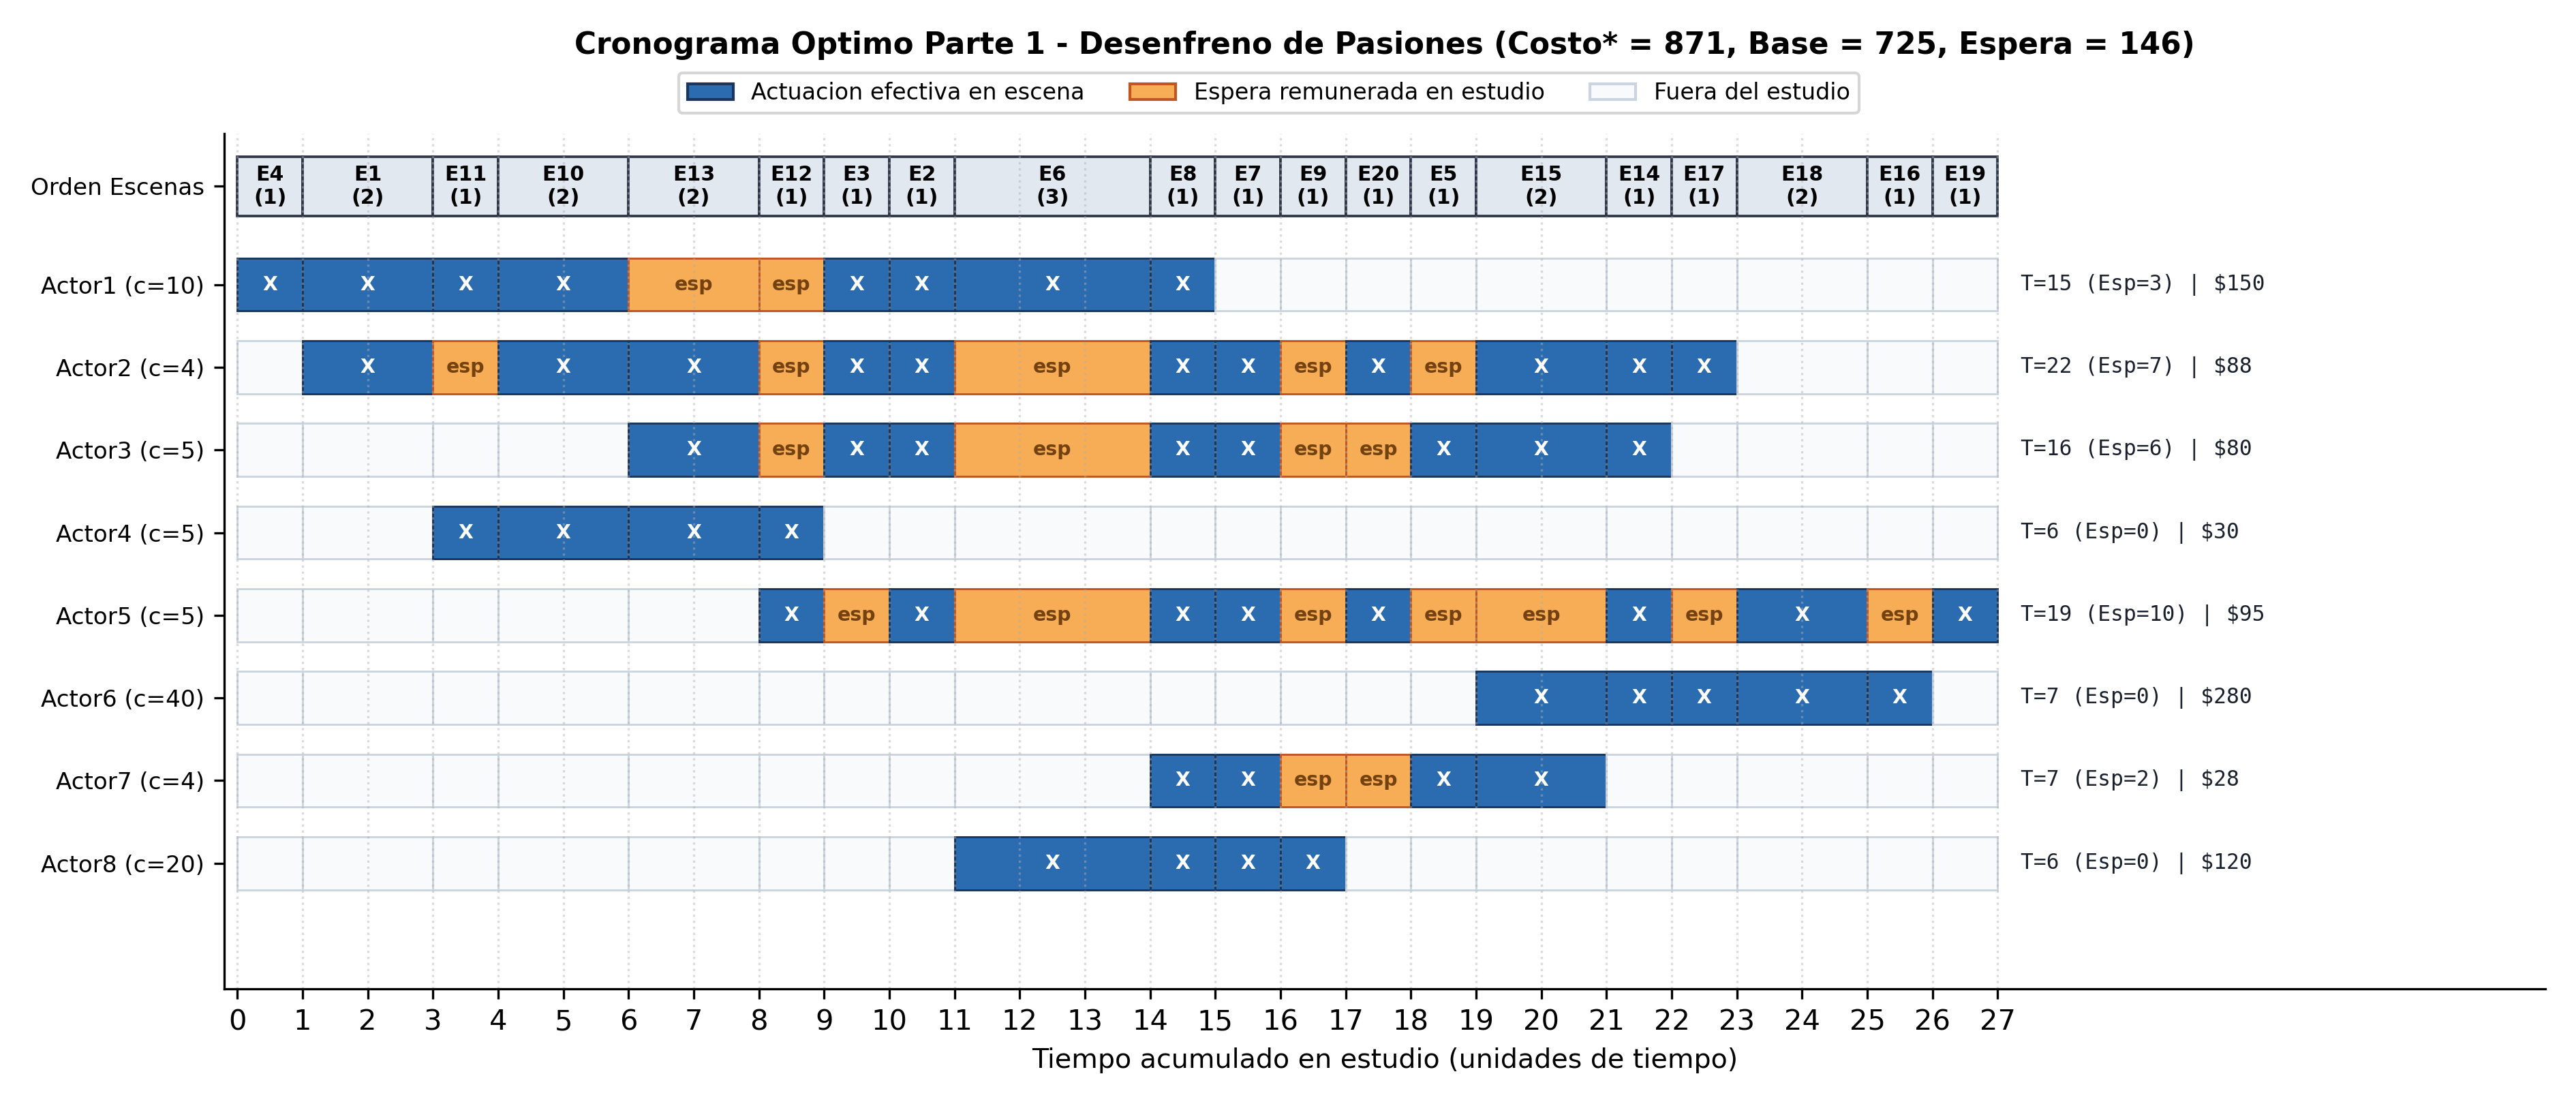
\includegraphics[width=0.90\textwidth]{parte1/gantt_desenfreno_p1.png}
    \caption{Cronograma óptimo de la Parte 1 (\texttt{Desenfreno2.dzn}): $Costo^* = 871$ ($C_{\text{fijo}} = 725$, espera $= 146$) con orden $(4, 1, 11, 10, 13, 12, 3, 2, 6, 8, 7, 9, 20, 5, 15, 14, 17, 18, 16, 19)$.}
    \label{fig:gantt_p1}
\end{figure}

\begin{figure}[!htbp]
    \centering
    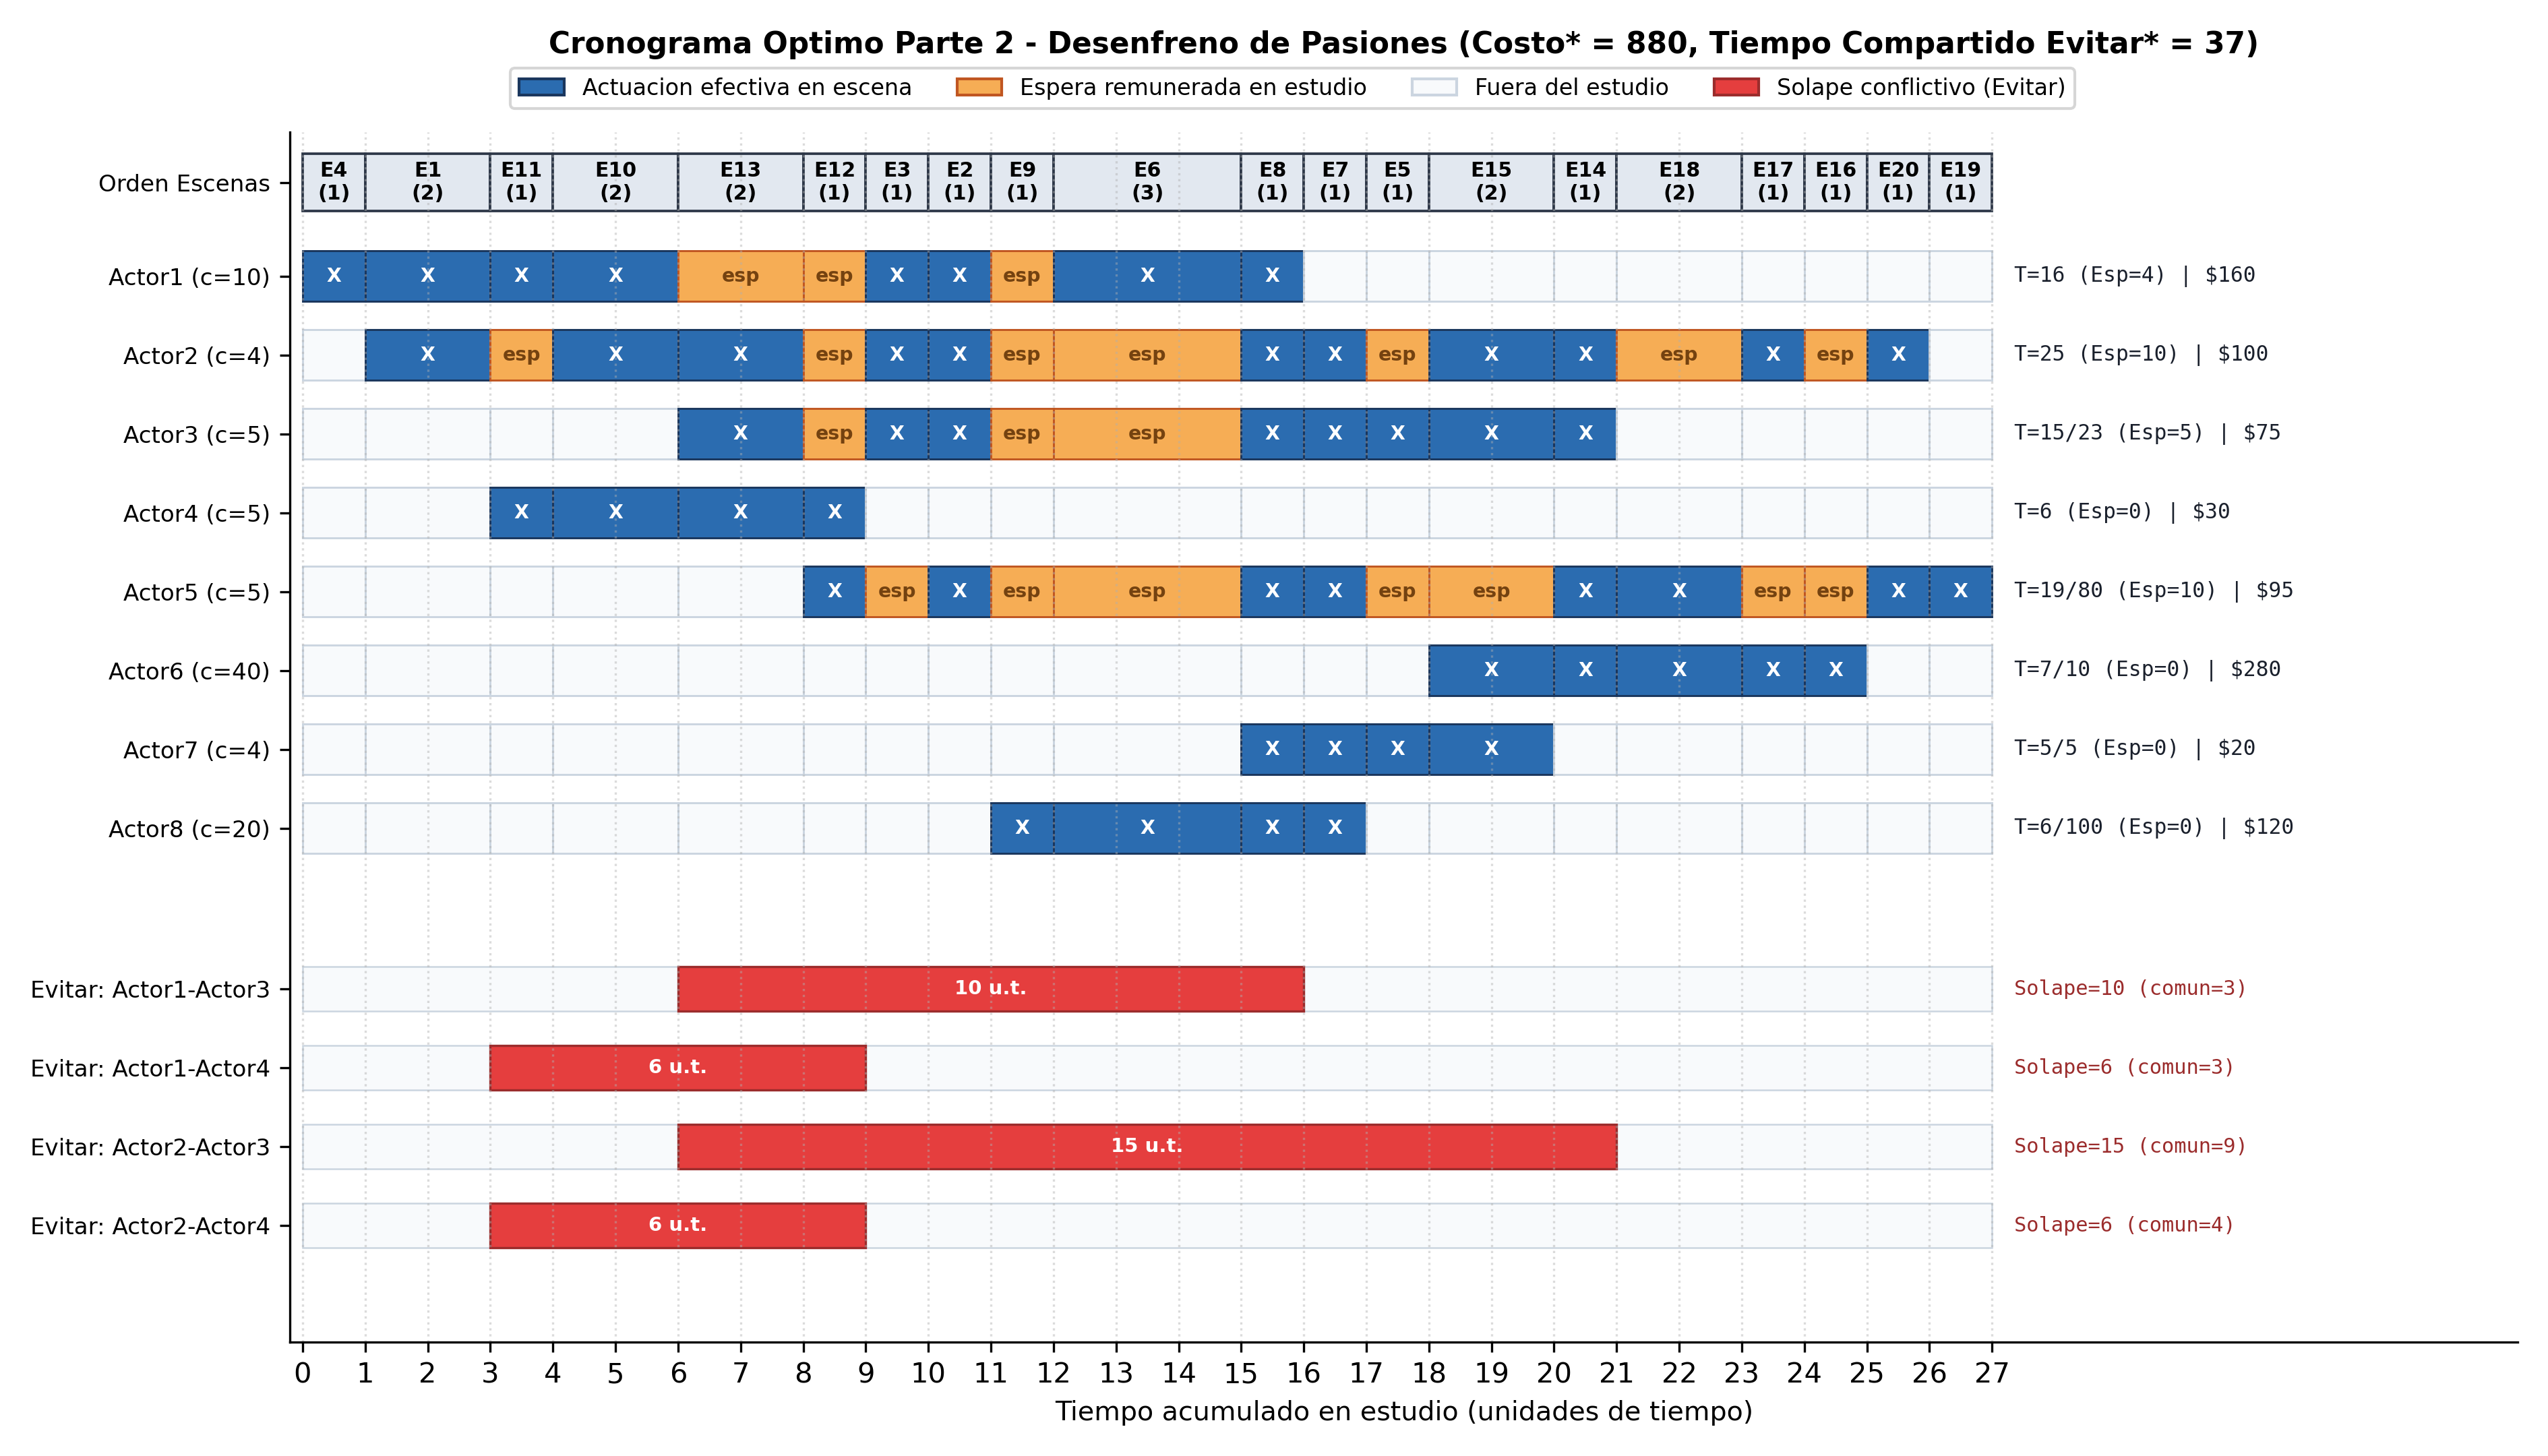
\includegraphics[width=0.90\textwidth]{parte2/gantt_desenfreno_p2_evitar.png}
    \caption{Cronograma óptimo de la Parte 2 (\texttt{Desenfreno4.dzn}): $Costo^* = 880$, $TC^* = 37$ con orden $(4, 1, 11, 10, 13, 12, 3, 2, 9, 6, 8, 7, 5, 15, 14, 18, 17, 16, 20, 19)$.}
    \label{fig:gantt_p2}
\end{figure}

\begin{figure}[!htbp]
    \centering
    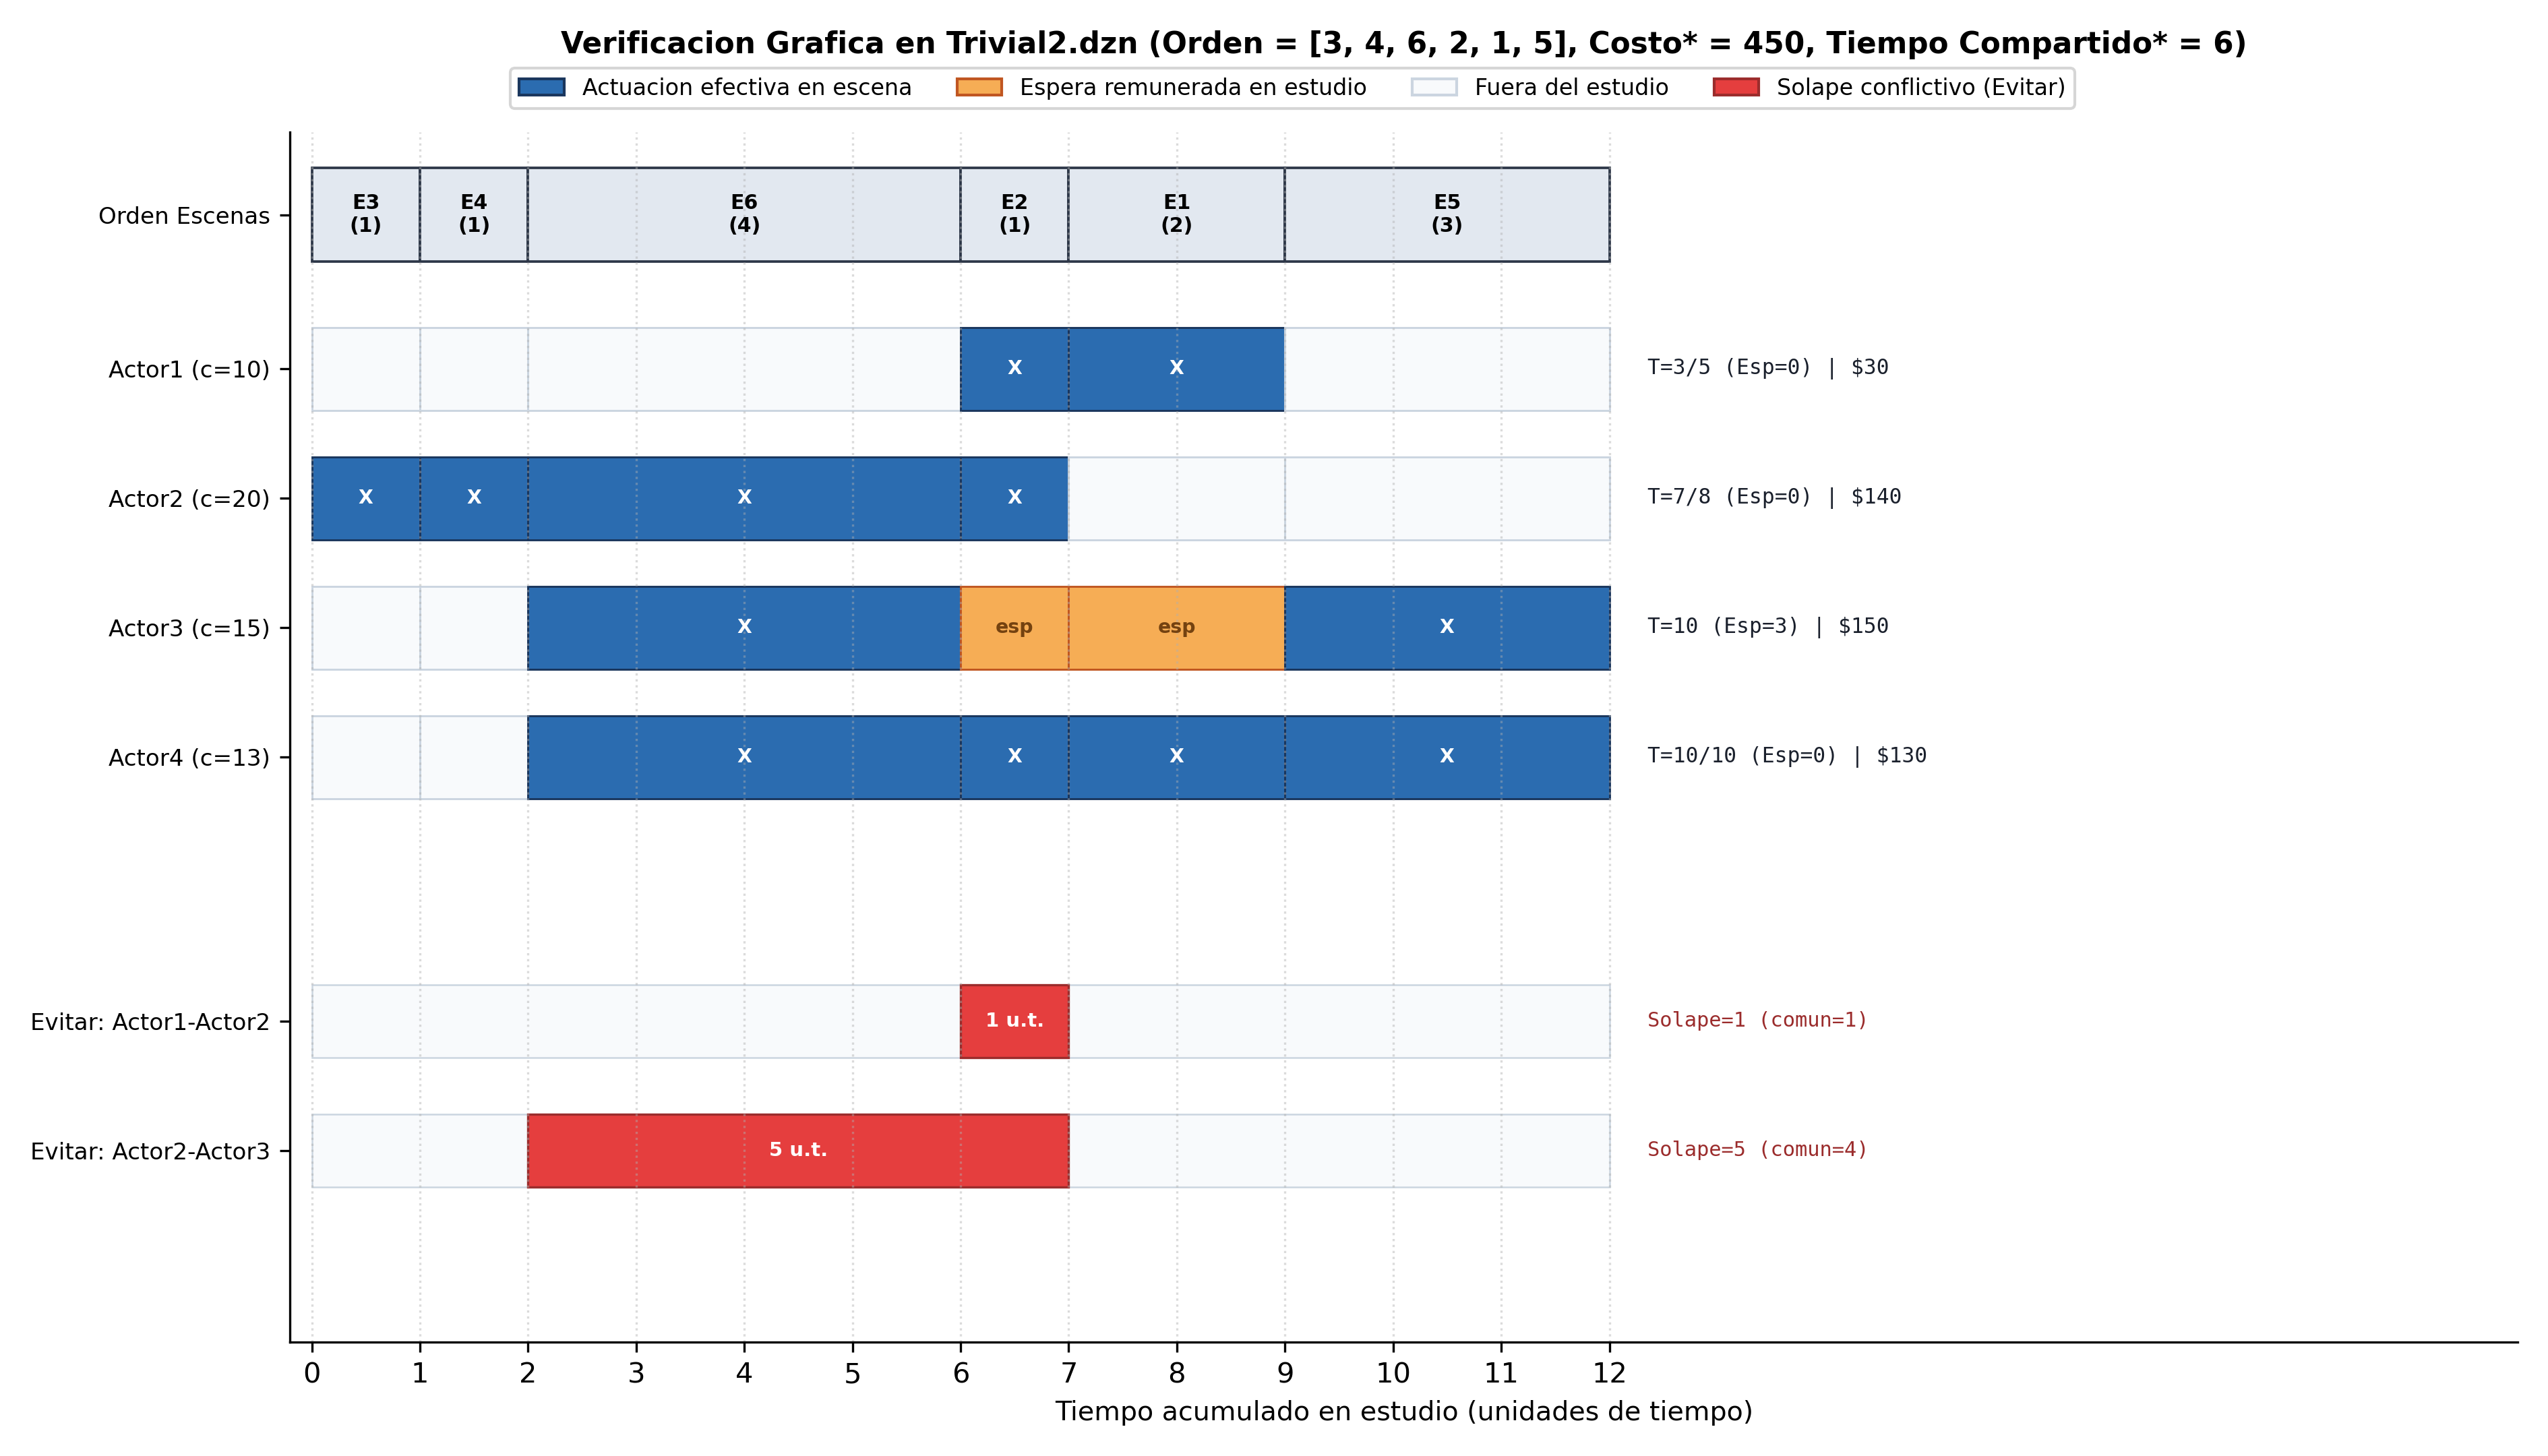
\includegraphics[width=0.86\textwidth]{parte2/verificacion_trivial2_p2.png}
    \caption{Caso base Parte 2 (\texttt{Trivial2.dzn}) con $(Costo^*, TC^*) = (450, 6)$; el orden canónico $(3, 4, 6, 2, 1, 5)$ equivale bajo $S_2$ a $(4, 3, 6, 2, 1, 5)$.}
    \label{fig:gantt_trivial2}
\end{figure}

\begin{itemize}
    \item \textbf{Efecto de \texttt{Disponibilidad}:} En \texttt{Desenfreno2} ($Costo^* = 871$, Figura~\ref{fig:gantt_p1}), los Actores 6 ($c_6 = 40$), 8 ($c_8 = 20$) y 4 ($c_4 = 5$) no tienen esperas, pero el Actor 7 permanece $T_7 = 7$ unidades (espera en $E_9$ y $E_{20}$). En \texttt{Desenfreno4} (Figura~\ref{fig:gantt_p2}), $Disp_7 = 5 = D^{\min}_7$ invalida dicho plan y fuerza a agrupar $[E_8, E_7, E_5, E_{15}]$ en $t \in [15, 20]$, desplazando $E_9$ a $[11, 12]$ y subiendo el óptimo exacto a $Costo^* = 880$ ($+9$ unidades, $\$900\,000$ pesos; análogo a \texttt{Instancia03}: $1531 \to 1544$).
    \item \textbf{Reducción de búsqueda en Parte 2 ($6{,}62\text{ s} \to 1{,}62\text{ s}$):} Pese a sumar variables y criterios, en ``Desenfreno de Pasiones'' los nodos caen $4{,}29\times$ ($71\,753 \to 16\,742$) y los fallos $4{,}45\times$ ($69\,264 \to 15\,582$) porque $R_3$ convierte $Disp_7 = 5$ y $Disp_6 = 10$ en cotas estrechas sobre $ultima_a - primera_a$ desde la raíz.
    \item \textbf{Composición de \texttt{Evitar}:} En \texttt{Desenfreno4}, $\underline{TC} = 3 + 3 + 9 + 4 = 19$ unidades corresponden a escenas compartidas obligatorias; las $18$ restantes hasta $TC^* = 37$ provienen de no separar los bloques de los Actores 1 y 4 respecto a 2 y 3 para no elevar $Costo$ por encima de $880$.
\end{itemize}

\subsection{Ablación: Simetrías vs.\ Modelo Original y Redundantes}

La Tabla~\ref{tab:ablacion} y las Figuras~\ref{fig:ablacion_p1}--\ref{fig:ablacion_p2} comparan el modelo primario original ($M_0$), solo simetrías ($M_1 = M_0 + S_1..S_3$), solo redundantes ($M_2 = M_0 + R_1..R_4$) y el modelo completo ($M_3$).

\begin{table}[!htbp]
\centering
\caption{Ablación ($M_0$ a $M_3$; \texttt{Gecode} para $M \le 12$, \texttt{Chuffed} con límite de $15\text{ s}$ para $M = 20$).}
\label{tab:ablacion}
\resizebox{\textwidth}{!}{%
\setlength{\tabcolsep}{2.8pt}
\begin{tabular}{llrrrrrrrrrrrr}
\toprule
& & \multicolumn{3}{c}{\textbf{$M_0$ (Original)}} & \multicolumn{3}{c}{\textbf{$M_1$ ($+S_1..S_3$)}} & \multicolumn{3}{c}{\textbf{$M_2$ ($+R_1..R_4$)}} & \multicolumn{3}{c}{\textbf{$M_3$ (Completo)}} \\
\cmidrule(lr){3-5} \cmidrule(lr){6-8} \cmidrule(lr){9-11} \cmidrule(lr){12-14}
\textbf{Instancia} & \textbf{Óptimo} & \textbf{Nodos} & \textbf{Fallos} & \textbf{T (s)} & \textbf{Nodos} & \textbf{Fallos} & \textbf{T (s)} & \textbf{Nodos} & \textbf{Fallos} & \textbf{T (s)} & \textbf{Nodos} & \textbf{Fallos} & \textbf{T (s)} \\
\midrule
\texttt{Trivial1}        & $255$       &       11 &       4 & 0,001 &       11 &       4 & 0,001 &        9 &       3 & 0,001 &      9 &      3 & 0,001 \\
\texttt{Instancia01\_P1} & $225$       &      443 &     219 & 0,002 &       26 &      10 & 0,001 &       71 &      32 & 0,001 &     18 &      6 & 0,001 \\
\texttt{Instancia02\_P1} & $871$       &   6\,535 &  3\,250 & 0,028 &   3\,699 &  1\,834 & 0,016 &   1\,136 &     548 & 0,012 &    606 &    286 & 0,007 \\
\texttt{Instancia03\_P1} & $1531$      & 374\,456 & 187\,201 & 1,566 & 181\,709 & 90\,831 & 0,761 &  74\,856 & 37\,400 & 0,667 & 36\,964 & 18\,457 & 0,333 \\
\texttt{Desenfreno2}     & $871$       & 209\,588$^\ddagger$ & 206\,922 & 14,79 & 207\,560$^\ddagger$ & 204\,772 & 14,79 & 121\,572 & 118\,466 & 12,35 & 71\,753 & 69\,264 & 6,596 \\
\midrule
\texttt{Trivial2}        & $(450,6)$   &       55 &      27 & 0,001 &       17 &       8 & 0,001 &       27 &      13 & 0,001 &     11 &      5 & 0,001 \\
\texttt{Instancia01\_P2} & $(225,5)$   &      348 &     165 & 0,002 &      232 &     107 & 0,002 &      220 &     101 & 0,002 &    148 &     65 & 0,002 \\
\texttt{Instancia02\_P2} & $(871,17)$  &   4\,125 &  2\,053 & 0,021 &   2\,637 &  1\,307 & 0,013 &      588 &     284 & 0,006 &    430 &    203 & 0,005 \\
\texttt{Instancia03\_P2} & $(1544,37)$ & 149\,505 & 74\,731 & 0,653 &  71\,767 & 35\,874 & 0,314 &  26\,202 & 13\,079 & 0,239 & 13\,059 &  6\,520 & 0,122 \\
\texttt{Desenfreno4}     & $(880,37)$  & 139\,661$^\ddagger$ & 136\,362 & 14,79 &  92\,992 & 90\,698 & 10,07 &  29\,302 & 27\,743 & 2,727 & 16\,742 & 15\,582 & 1,572 \\
\bottomrule
\multicolumn{14}{l}{\footnotesize $^\ddagger$Halla el valor óptimo pero agota $15\text{ s}$ sin certificar optimalidad.}
\end{tabular}%
}
\end{table}

\begin{figure}[!htbp]
    \centering
    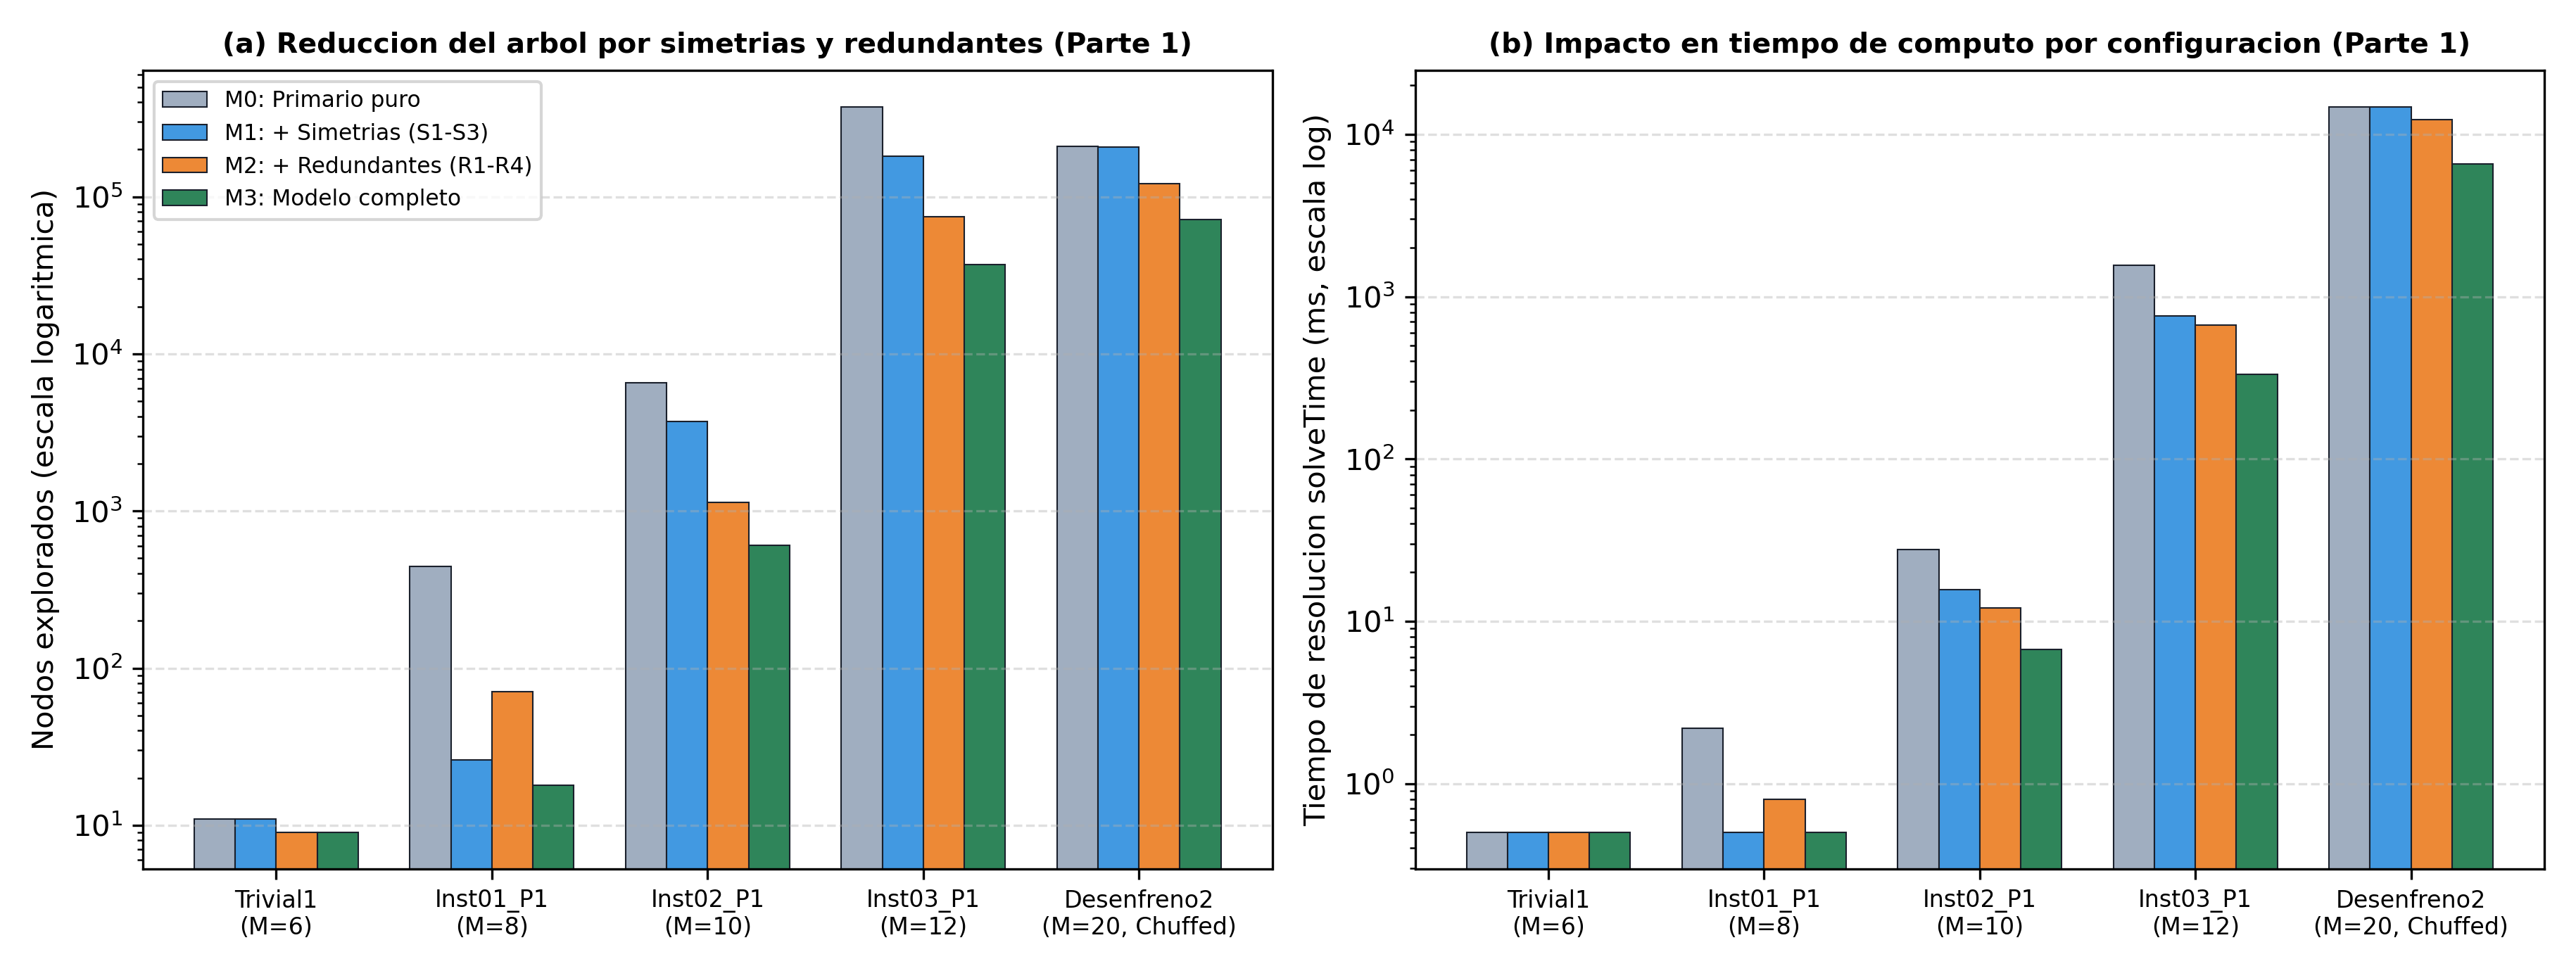
\includegraphics[width=0.83\textwidth]{parte1/ablacion_poda_p1.png}
    \caption{Efecto de las simetrías ($S_1$--$S_3$) y redundantes ($R_1$--$R_4$) sobre nodos y tiempos en la Parte 1.}
    \label{fig:ablacion_p1}
\end{figure}

\begin{figure}[!htbp]
    \centering
    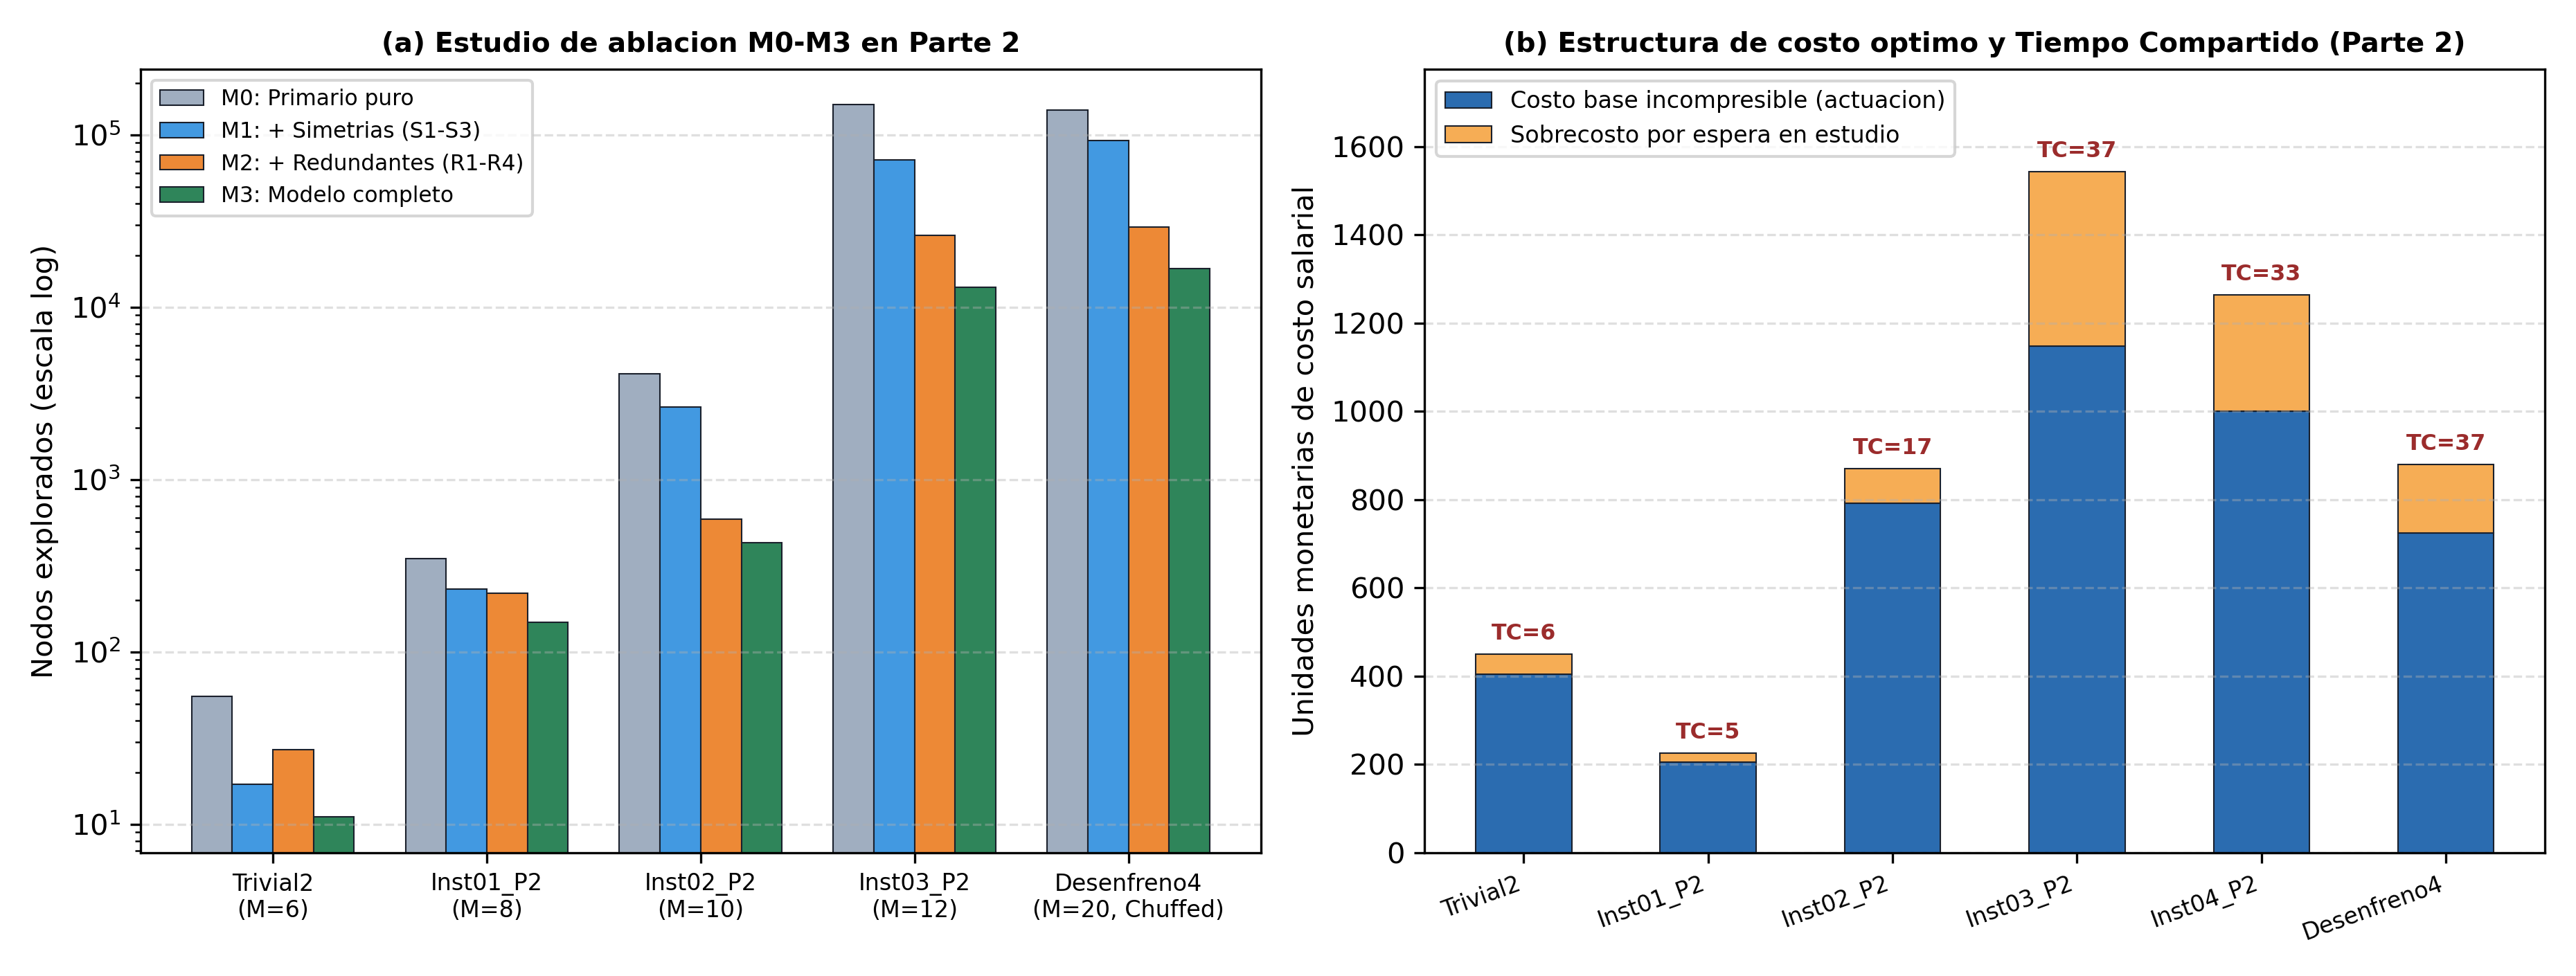
\includegraphics[width=0.83\textwidth]{parte2/ablacion_y_tradeoff_p2.png}
    \caption{Ablación en la Parte 2 y descomposición entre $C_{\text{fijo}}$, espera y tiempo compartido (\texttt{Evitar}).}
    \label{fig:ablacion_p2}
\end{figure}

\begin{itemize}
    \item \textbf{Aporte de simetrías ($M_0 \to M_1$, $M_2 \to M_3$):} Donde solo actúa $S_1$ (\texttt{Instancia03\_P1/P2}), los nodos y fallos se reducen a la mitad ($374\,456 \to 181\,709$, $-51{,}5\%$; $149\,505 \to 71\,767$, $-52{,}0\%$). Con escenas vacías y gemelas, $M_1$ reduce el árbol $17{,}04\times$ en \texttt{Instancia01\_P1} ($443 \to 26$ nodos) y $3{,}24\times$ en \texttt{Trivial2} ($55 \to 17$), y en \texttt{Desenfreno4} logra certificar optimalidad en $10{,}07\text{ s}$ frente al corte por tiempo de $M_0$.
    \item \textbf{Combinación con redundantes ($M_3$):} En \texttt{Desenfreno2}, $M_0$ y $M_1$ agotan $15\text{ s}$ sin prueba de optimalidad; $R_1$--$R_4$ ($M_2$) cierran la prueba en $12{,}35\text{ s}$ y $M_3$ la baja a $6{,}60\text{ s}$, con reducciones totales de $24{,}61\times$ (\texttt{Instancia01\_P1}), $10{,}13\times$ (\texttt{Instancia03\_P1}), $11{,}45\times$ (\texttt{Instancia03\_P2}) y $8{,}34\times$ en nodos ($9{,}41\times$ en tiempo) sobre \texttt{Desenfreno4}.
\end{itemize}

\subsection{Comparación de Estrategias de Búsqueda (\texorpdfstring{$E_1$--$E_8$}{E1-E8})}

La Tabla~\ref{tab:estrategias} y la Figura~\ref{fig:estrategias} contrastan $E_1$--$E_8$ con límite de $8{,}5\text{ s}$ por corrida.

\begin{table}[!htbp]
\centering
\caption{Comparación de las estrategias $E_1$--$E_8$ en $M=12$ (\texttt{Gecode} y \texttt{Chuffed}) y $M=20$ (\texttt{Chuffed}, límite $8{,}5\text{ s}$).}
\label{tab:estrategias}
\resizebox{\textwidth}{!}{%
\setlength{\tabcolsep}{2.4pt}
\begin{tabular}{llrrrrrrrrrrrrrr}
\toprule
& & \multicolumn{3}{c}{\textbf{Inst03\_P1 (Gecode)}} & \multicolumn{3}{c}{\textbf{Inst03\_P1 (Chuffed)}} & \multicolumn{4}{c}{\textbf{Desenfreno2 (Chuffed)}} & \multicolumn{4}{c}{\textbf{Desenfreno4 (Chuffed)}} \\
\cmidrule(lr){3-5} \cmidrule(lr){6-8} \cmidrule(lr){9-12} \cmidrule(lr){13-16}
\textbf{ID} & \textbf{Estrategia} & \textbf{Nodos} & \textbf{Fallos} & \textbf{T (s)} & \textbf{Nodos} & \textbf{Fallos} & \textbf{T (s)} & \textbf{Costo} & \textbf{Nodos} & \textbf{Fallos} & \textbf{T (s)} & \textbf{Par} & \textbf{Nodos} & \textbf{Fallos} & \textbf{T (s)} \\
\midrule
$E_1$ & Out-In Peso Asc    &  36\,964 &  18\,457 & 0,335 &  4\,049 &  3\,786 & 0,147 & \textbf{871}$\checkmark$ &  71\,753 & 69\,264 & \textbf{6,676} & \textbf{(880,37)}$\checkmark$ &  16\,742 & 15\,582 & \textbf{1,592} \\
$E_2$ & Out-In ID Nominal  &  47\,716 &  23\,809 & 0,375 &  5\,650 &  5\,166 & 0,195 & 871$^*$                  &  98\,608 & 94\,538 & 8,262          & (880,37)$\checkmark$          &  40\,289 & 38\,085 & 3,916 \\
$E_3$ & Izquierda-Derecha  & 785\,034$^*$ & 392\,451 & 8,290 & 66\,907 & 66\,234 & 4,282 & 925$^*$              &  71\,174 & 70\,841 & 8,275          & (899,45)$^*$                  &  63\,829 & 62\,550 & 8,278 \\
$E_4$ & First-Fail + Min   & 440\,476 & 220\,173 & 4,230 & 22\,645 & 21\,971 & 1,126 & 925$^*$                  &  72\,526 & 71\,788 & 8,281          & (880,37)$\checkmark$          &  75\,862 & 73\,078 & 8,023 \\
$E_5$ & First-Fail + Split & 438\,673 & 219\,270 & 3,829 & 26\,767 & 23\,648 & 1,249 & 925$^*$                  &  78\,591 & 65\,207 & 8,276          & (880,37)$\checkmark$          &  85\,669 & 72\,754 & 7,834 \\
$E_6$ & Pos Costo + Med    & 582\,417$^*$ & 291\,174 & 8,292 & 94\,318$^*$ & 93\,915 & 8,277 & 1049$^*$          &  77\,915 & 76\,985 & 8,280          & (970,41)$^*$                  &  70\,750 & 69\,748 & 8,272 \\
$E_7$ & Dom/WDeg Out-In    &  36\,956 &  18\,453 & 0,337 &  4\,049 &  3\,786 & 0,147 & \textbf{871}$\checkmark$ &  71\,753 & 69\,264 & 6,714          & \textbf{(880,37)}$\checkmark$ &  16\,742 & 15\,582 & 1,538 \\
$E_8$ & Default Solver     & 146\,445 &  73\,167 & 1,168 & 161\,833$^*$ & 116\,481 & 8,295 & 1046$^*$           & 143\,053 & 87\,742 & 8,281          & (1094,48)$^*$                 & 132\,022 & 76\,344 & 8,279 \\
\bottomrule
\multicolumn{16}{l}{\footnotesize $\checkmark$ Optimalidad certificada (\texttt{==========}). \quad $^*$Agota $8{,}5\text{ s}$ sin certificar optimalidad.}
\end{tabular}%
}
\end{table}

\begin{figure}[!htbp]
    \centering
    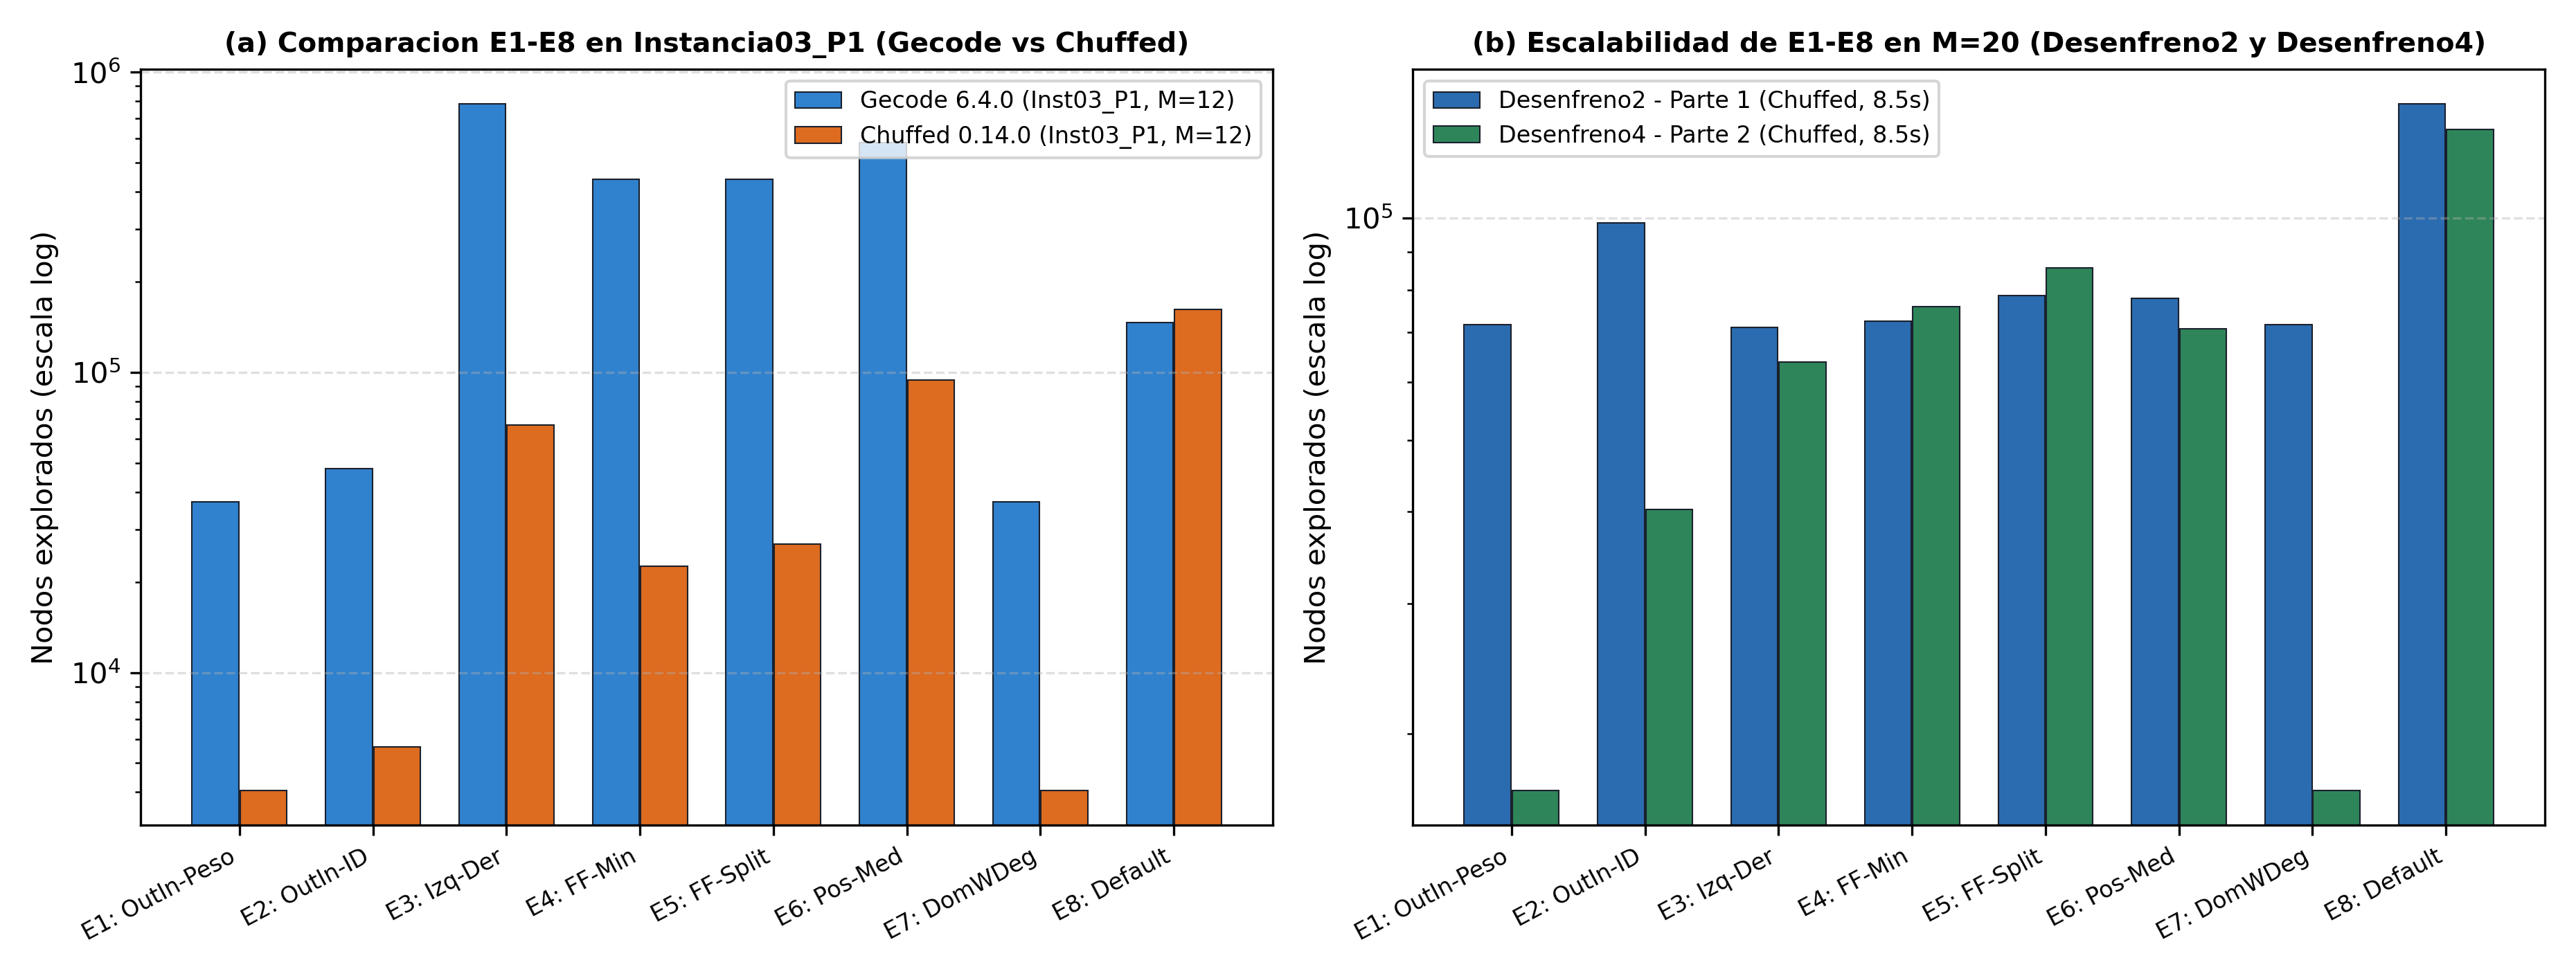
\includegraphics[width=0.82\textwidth]{parte1/estrategias_busqueda_p1.png}
    \caption{Nodos explorados por las estrategias $E_1$--$E_8$ en $M=12$ (\texttt{Gecode} y \texttt{Chuffed}) y $M=20$ (\texttt{Chuffed}).}
    \label{fig:estrategias}
\end{figure}

\begin{itemize}
    \item \textbf{Limitación de la búsqueda por defecto ($E_8$):} En \texttt{Gecode} explora $3{,}96\times$ más nodos y fallos que $E_1$; en \texttt{Chuffed} agota el tiempo incluso en $M=12$, y en $M=20$ se estanca en $Costo = 1046$ (\texttt{Desenfreno2}) y $(1094, 48)$ (\texttt{Desenfreno4}), lejos de $871$ y $(880, 37)$.
    \item \textbf{Efecto del orden \emph{Outside-In} ($E_3 \to E_2$) y del peso salarial ($E_2 \to E_1$):} Pasar de izquierda-a-derecha ($E_3$) a extremos intercalados ($E_2$) en \texttt{Instancia03\_P1} reduce $11{,}84\times$ los nodos y $21{,}96\times$ el tiempo en \texttt{Chuffed}. Ordenar además los valores por $W_e$ ascendente ($E_1$, igualada por $E_7$) recorta $2{,}41\times$ los nodos en \texttt{Desenfreno4} ($40\,289 \to 16\,742$) y permite certificar \texttt{Desenfreno2} en $6{,}68\text{ s}$.
    \item \textbf{\texttt{Chuffed} vs.\ \texttt{Gecode}:} Distintos prefijos y sufijos generan el mismo conjunto de actores abiertos en el bloque central; mientras \texttt{Gecode} re-explora subárboles equivalentes por DFS (razón nodos/fallos $\approx 2{:}1$), \texttt{Chuffed} aprende cláusulas \emph{nogood} sobre literales de orden e intermediación, reduciendo entre $9\times$ y $46\times$ los nodos para $M \ge 12$.
\end{itemize}

% !TEX root = ../main.tex
\section{Conclusiones}
\label{sec:conclusiones}

El análisis matemático, el desarrollo declarativo en \texttt{MiniZinc} de los modelos de Parte 1 y Parte 2 adherido rigurosamente a los fundamentos del curso, la construcción de la interfaz gráfica y normalizada de entrada/salida y la experimentación exhaustiva sobre trece instancias permiten establecer las siguientes conclusiones técnicas debidamente sustentadas:

\begin{enumerate}
    \item \textbf{Idoneidad de la canalización primal-dual sin salir del núcleo declarativo del curso:}
    Representar simultáneamente el cronograma mediante el arreglo por turnos $Orden_k$ y su permutación inversa por escenas $Pos_e$ a través del predicado global \texttt{inverse}, acoplados con un vector de tiempos acumulados $Acum_k$, permite expresar el ingreso, el retiro y la estadía continua de cada actor empleando únicamente agregadores \texttt{min}, \texttt{max} y restricciones \texttt{element} sobre conjuntos estáticos de escenas propias $E_a$, mientras todo el preprocesamiento de rangos salariales y duraciones ordenadas se resuelve con listas por comprensión y sumas aritméticas elementales. Esta arquitectura evita tanto la multiplicación cuadrática de variables como la reificación superflua sobre las restricciones primarias ($C_1$--$C_5$).

    \item \textbf{Exactitud y eficiencia de la escalarización lexicográfica en optimización jerárquica:}
    En la Parte 2, el requerimiento de minimizar como criterio secundario la coincidencia en el estudio de los actores incluidos en \texttt{Evitar} sin deteriorar bajo ninguna circunstancia el costo salarial mínimo se resuelve de forma exacta en una única ejecución mediante la función lineal $ObjetivoLex = (\overline{TC} + 1)\cdot Costo + TiempoCompartido$. La contrastación contra el oráculo independiente confirma que esta formulación garantiza prioridad lexicográfica absoluta y mantiene dominios enteros reducidos libres de desbordamiento numérico.

    \item \textbf{Impacto decisivo y complementario de la eliminación de simetrías y las restricciones redundantes:}
    La comparación experimental directa frente al modelo primario original ($M_0$) demuestra que romper la inversión temporal sobre las escenas activas ($S_1$), ordenar escenas gemelas ($S_2$) y fijar en prefijo las escenas sin actores ($S_3$) preserva intacto el valor óptimo (permitiendo reconstruir algebraicamente toda la órbita de soluciones equivalentes descartadas) mientras poda más del $51\%$ de los nodos explorados y fallidos en instancias asimétricas generales y hasta un $94{,}1\%$ ($17{,}04\times$ por simetrías solas y $24{,}61\times$ en conjunto) cuando coexisten escenas vacías y gemelas (\texttt{Instancia01\_P1}). A su vez, las restricciones redundantes de intermediación lineal con coeficientes constantes ($R_1$), diferencias temporales entre subintervalos ($R_2$), amplitud posicional ($R_3$) y exceso mínimo ($R_4$) reducen conjuntamente los nodos explorados y fallidos en $10{,}13\times$ (\texttt{Instancia03\_P1}) y $11{,}45\times$ (\texttt{Instancia03\_P2}), haciendo posible certificar la optimalidad global de ``Desenfreno de Pasiones'' ($M=20$, $2{,}43 \times 10^{18}$ permutaciones) tanto en la Parte 1 ($Costo^* = 871$ en $6{,}60\text{ s}$) como en la Parte 2 ($Costo^* = 880, TC^* = 37$ en $1{,}57\text{ s}$).

    \item \textbf{Necesidad crítica de alinear la estrategia de distribución con la topología del acoplamiento temporal:}
    El análisis estadístico sobre nodos explorados, nodos fallidos y tiempos de respuesta de las ocho estrategias ($E_1$--$E_8$) evidencia que las heurísticas genéricas (cronológica izquierda-a-derecha $E_3$, \emph{first-fail} $E_4$--$E_5$ o la búsqueda libre por defecto del motor $E_8$, la cual queda estancada en costos altamente subóptimos de $1046$ en Parte 1 y $1094$ en Parte 2) sufren una degradación severa al crecer $M$, dado que dejan abiertos los extremos de permanencia actoral hasta niveles profundos del árbol. En contraste, instanciar las posiciones desde ambos extremos hacia el centro (\emph{Outside-In}) probando primero las escenas de menor peso salarial ($E_1$ y $E_7$) activa la ruptura de simetría $S_1$ en profundidad $2$, cierra tempranamente los intervalos actorales y descubre incumbentes casi óptimos desde las primeras ramas, consolidándose junto con el aprendizaje de cláusulas de \texttt{Chuffed} como la estrategia superior en toda la batería evaluada.
\end{enumerate}


\end{document}
